\subsection{\texorpdfstring{$ttZ$}{TTZ} background estimation}

  One of our main backgrounds in the \mtll tail is $t\bar{t}Z$, in which the $Z$-boson decays into neutrinos. These neutrinos add additional missing energy to the event which promotes $t\bar{t}Z$ events
  from to bulk into the tail of the \mtll distribution. We use two complementary methods to verify the cross section normalization and \mtll shape description respectively.

  \subsubsection{Normalization in the \texorpdfstring{$t\bar{t}Z \to 3l$}{ttZ->3l} region}

    The normalization of the $t\bar{t}Z$ background could be estimated in a data-driven way using the $3l$ sideband, in which the \Z decays into two leptons, one top decays leptonically and the other hadronically:
    \begin{equation}
      t\bar{t}Z \to (bl\nu) (bjj) (ll) \nonumber 
    \end{equation}

    This measurement has recently performed~\citep{CMS-PAS-TOP-16-017}, measuring a signal strength parameter of 
    \begin{equation}
     0.89^{+0.18}_{-0.16} \text{(stat) }^{+0.14}_{-0.12}\text{(sys)}
    \end{equation}
    We use the measured
    signal strength as a scale factor for the $t\bar{t}Z$ MC and propagate its statistical and systematic errors into our analysis.
    The measurement requires the presence of three leptons exceeding respectively \pt thresholds of 30, 20 and 10 GeV.
    Two of these leptons are required to have the same flavour and opposite charge and should fall within a $Z$-mass window of 10 GeV in order to construct the $Z$-boson candidate.
    Additionally, we require at least three jets of which at least one has been identified as a $b$-jet.
    Figure~\ref{fig:ttz3l} shows the dilepton mass and b-jet distribution.

%    \begin{figure}
%      \centering
%      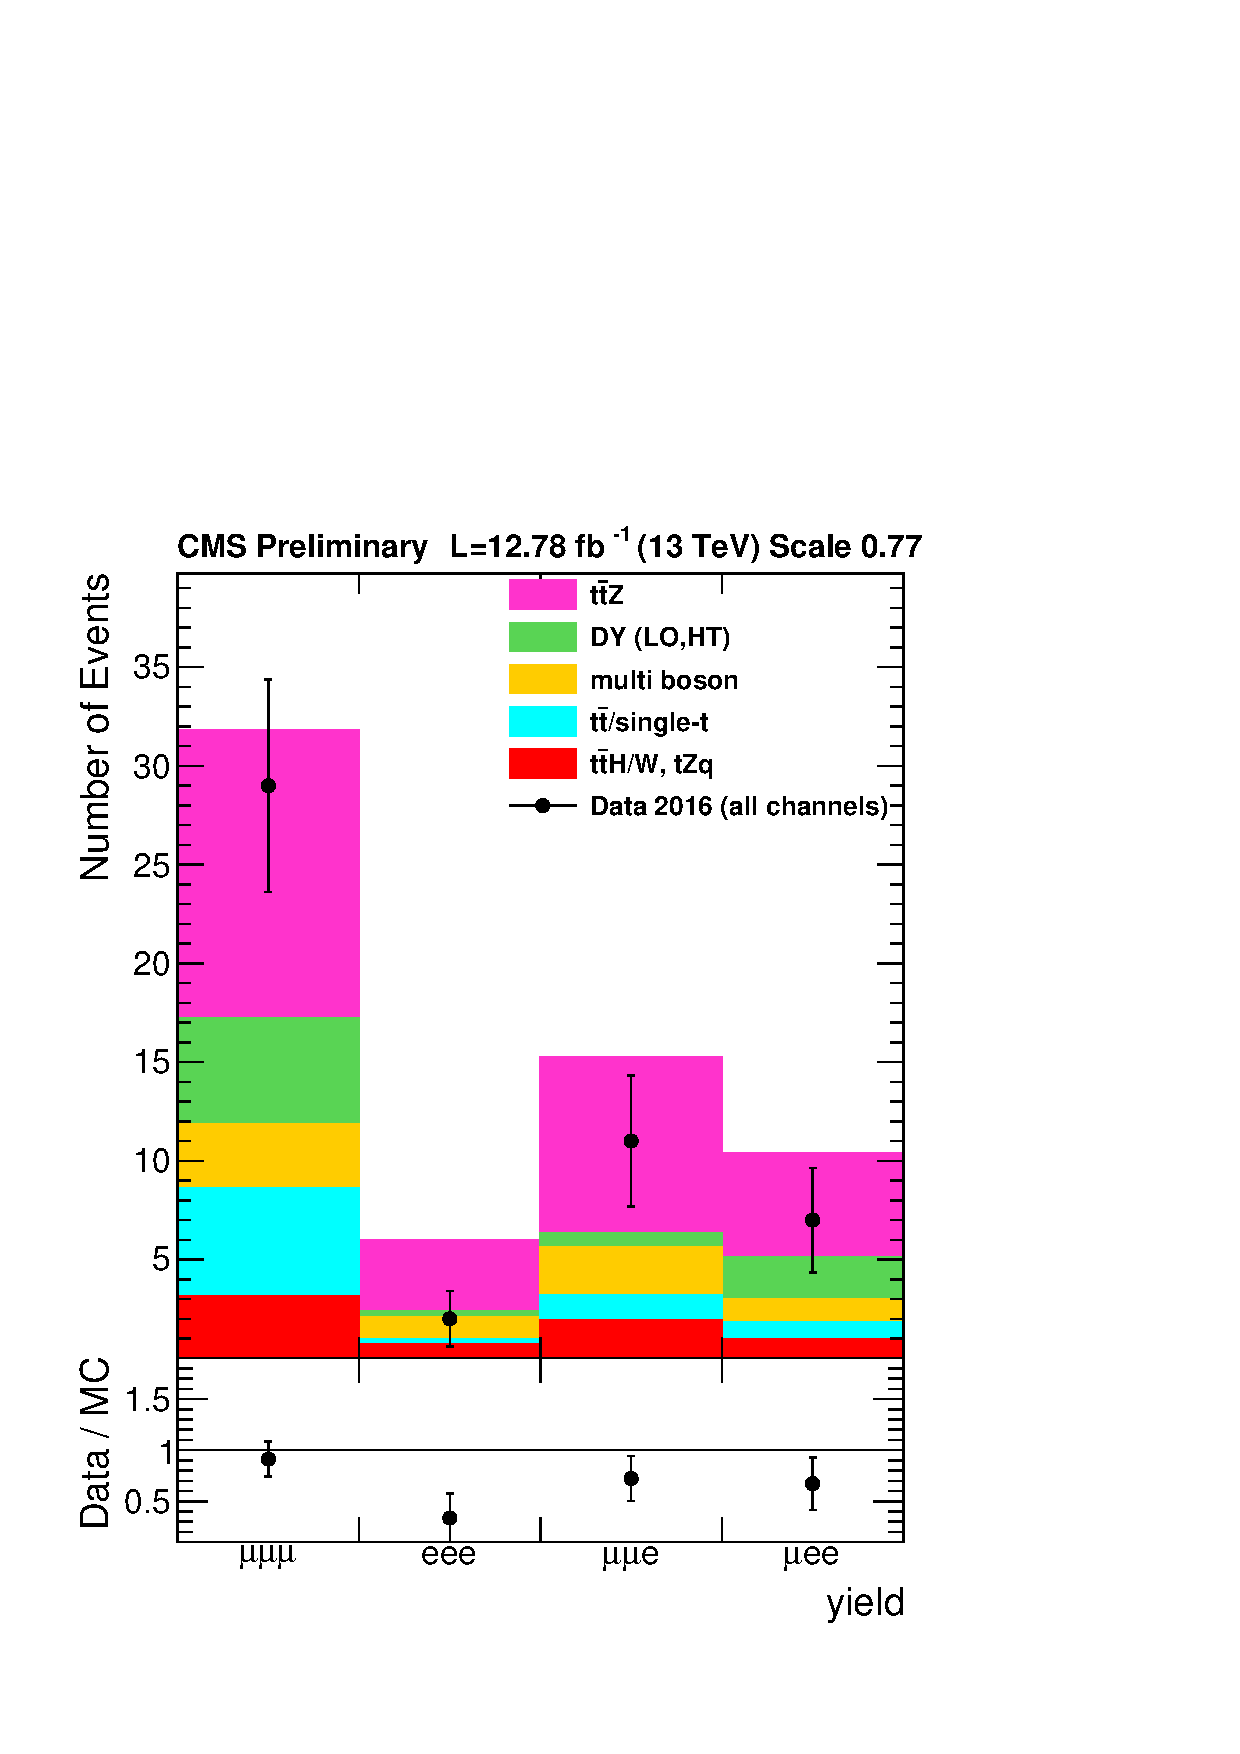
\includegraphics[width=0.7\textwidth]{figures/TTZ/all/njet3-nbtagLL-onZ-dR/yield.pdf}
%      \caption{Yields of the $t\bar{t}Z$ selection for the different 3-lepton channels}
%      \label{fig:ttz3l}
%    \end{figure}

    \begin{figure}
      \centering
      \includegraphics[width=0.45\textwidth]{figures/TOP-16-017/mll.png}
      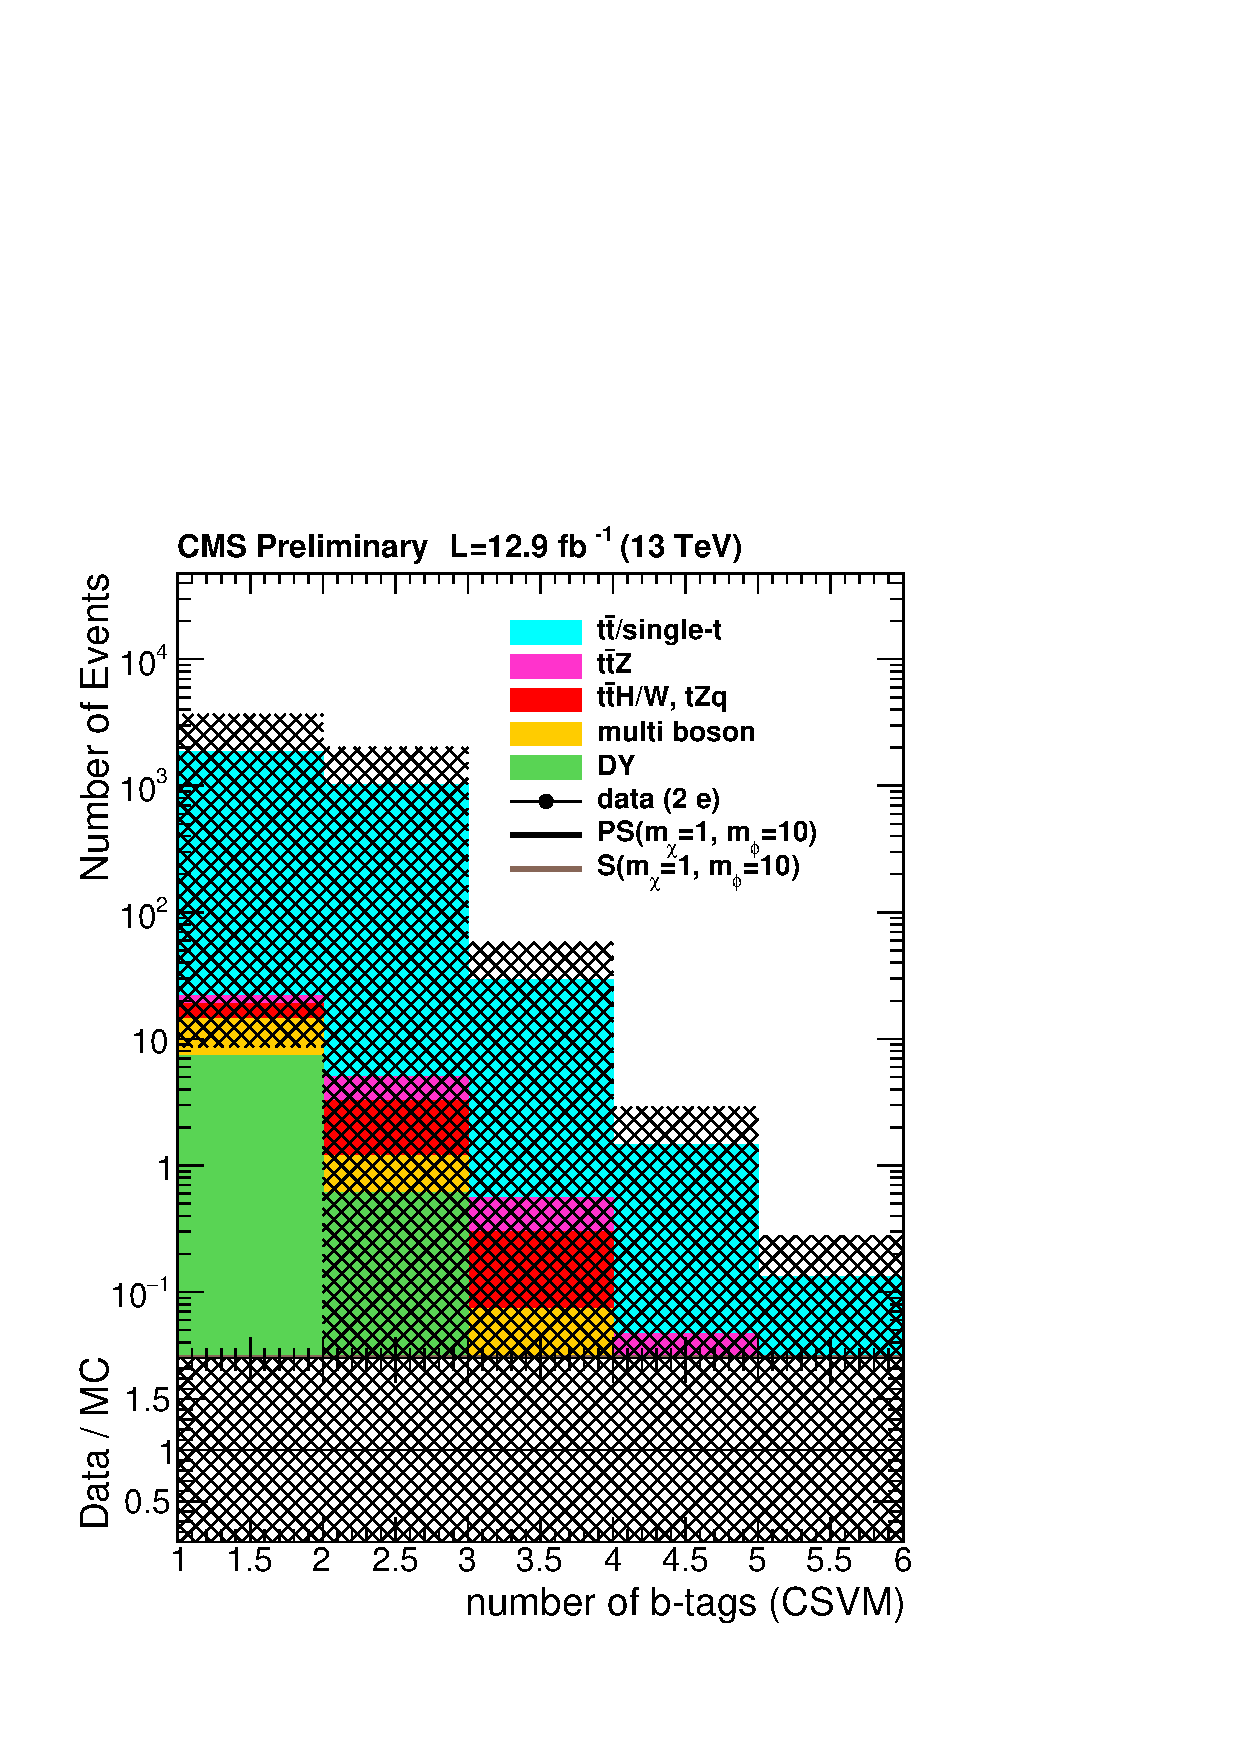
\includegraphics[width=0.45\textwidth]{figures/TOP-16-017/nbtags.png}
      \caption{Dilepton mass and b-jet distribution in the $t\bar{t}Z$ control region~\citep{CMS-PAS-TOP-16-017}}
      \label{fig:ttz3l}
    \end{figure}


  \subsubsection{Shape control region using \texorpdfstring{$tt\gamma$}{ttg} events}
    In order to verify the MC description of the \met and \mtll tails for the $t\bar{t}Z$ background, we select $t\bar{t}\gamma$ events in data and treat the photon \pt as additional missing energy
    such that it acts as a proxy for $t\bar{t}Z$ (\ie the photon \pt is vectorially added to the \met). Photons are selected according to Tab.~\ref{photonSelection}. Even though the kinematics of $t\bar{t}\gamma$ events differ from $t\bar{t}Z$ events due to the fact that the photon is massless, these kinematic
    differences could be mitigated by a reweighting of the boson \pt. Figure~\ref{fig:ttgGen} shows that the \met, \mtll, \mtlblb and \mtbb variables at generator-level between $t\bar{t}\gamma$ and $t\bar{t}Z$ are very similar
    after a bin-by-bin reweighting of the photon \pt to the $Z$ boson \pt,

    % GEN plots
    \begin{figure}
      \centering
      \subfloat[]{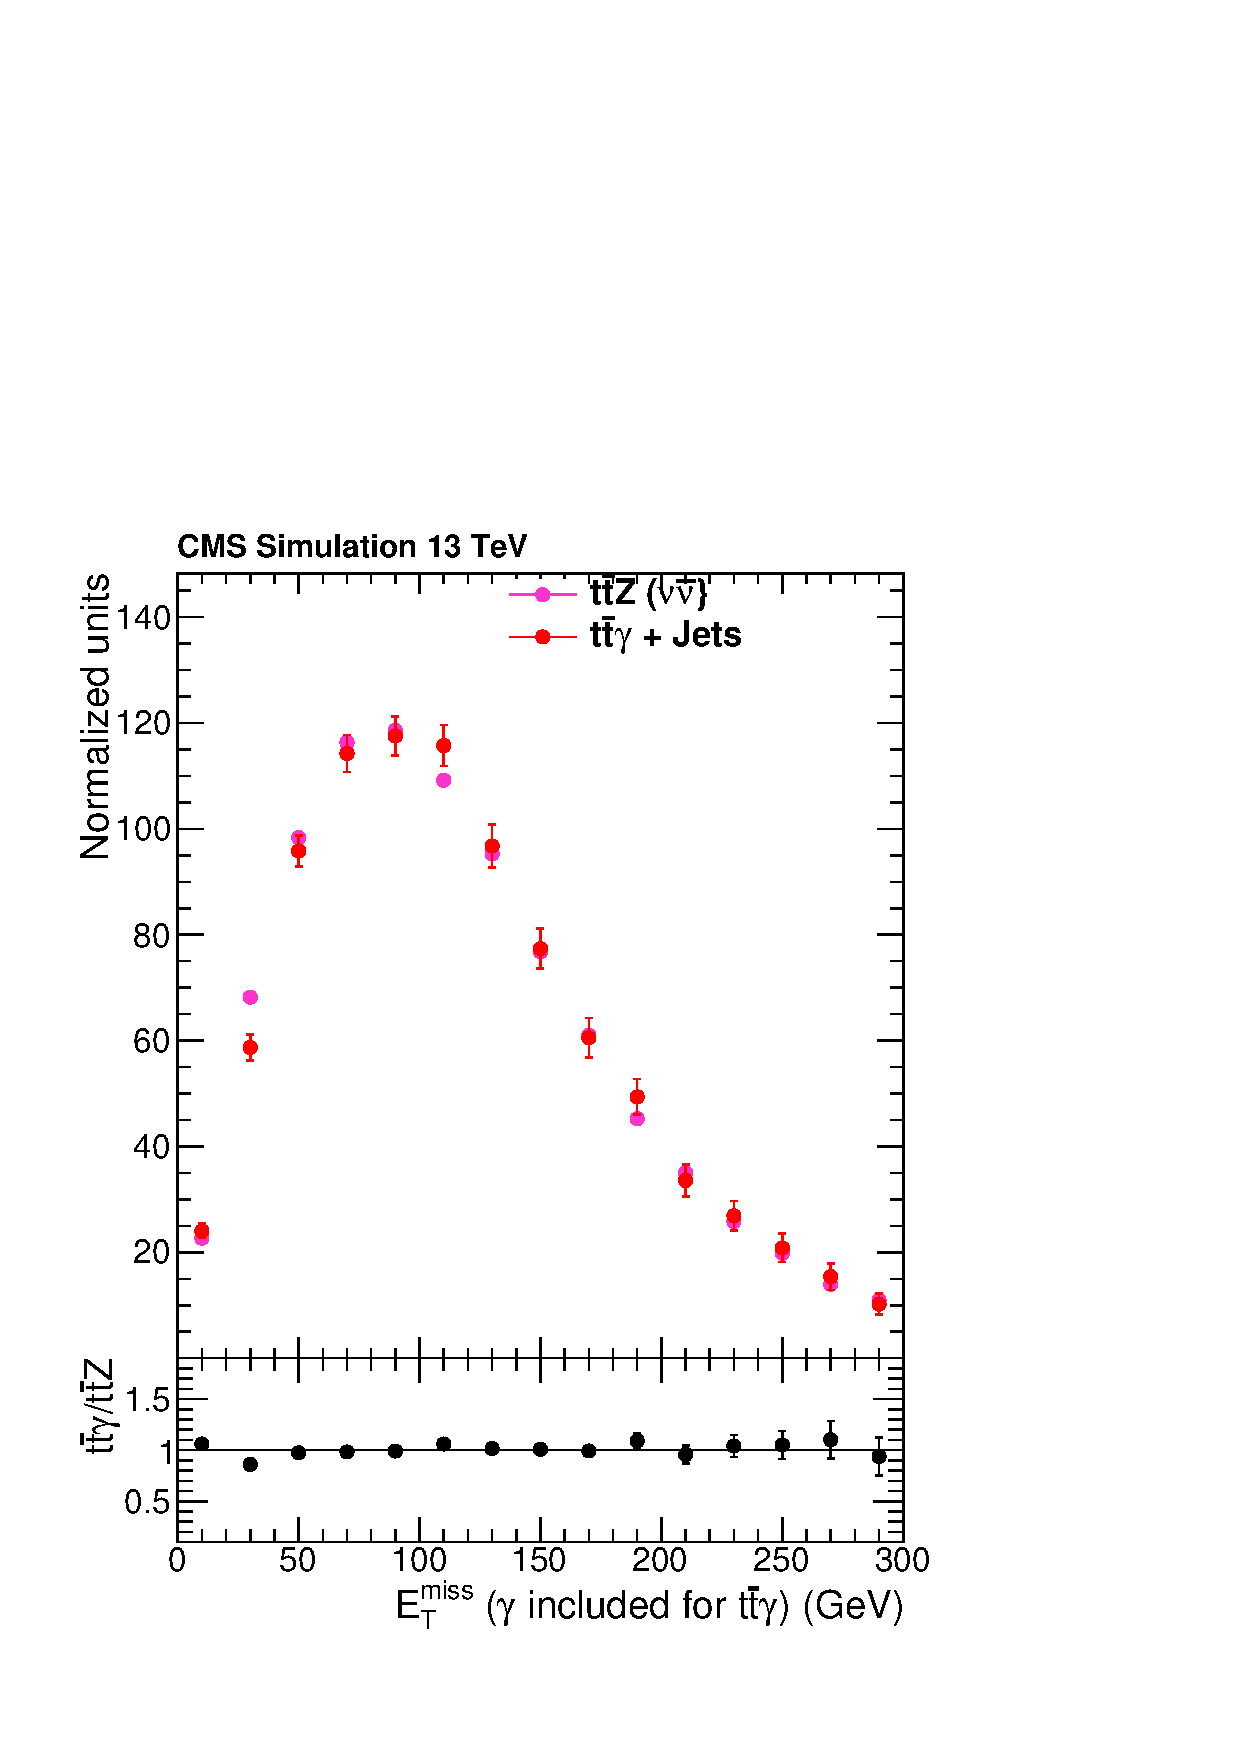
\includegraphics[width=0.45\textwidth]{figures/TTG_gen/reweighted/all_normalized/etaGamma25-ptGamma30/met_photonIncluded.pdf}}
      \subfloat[]{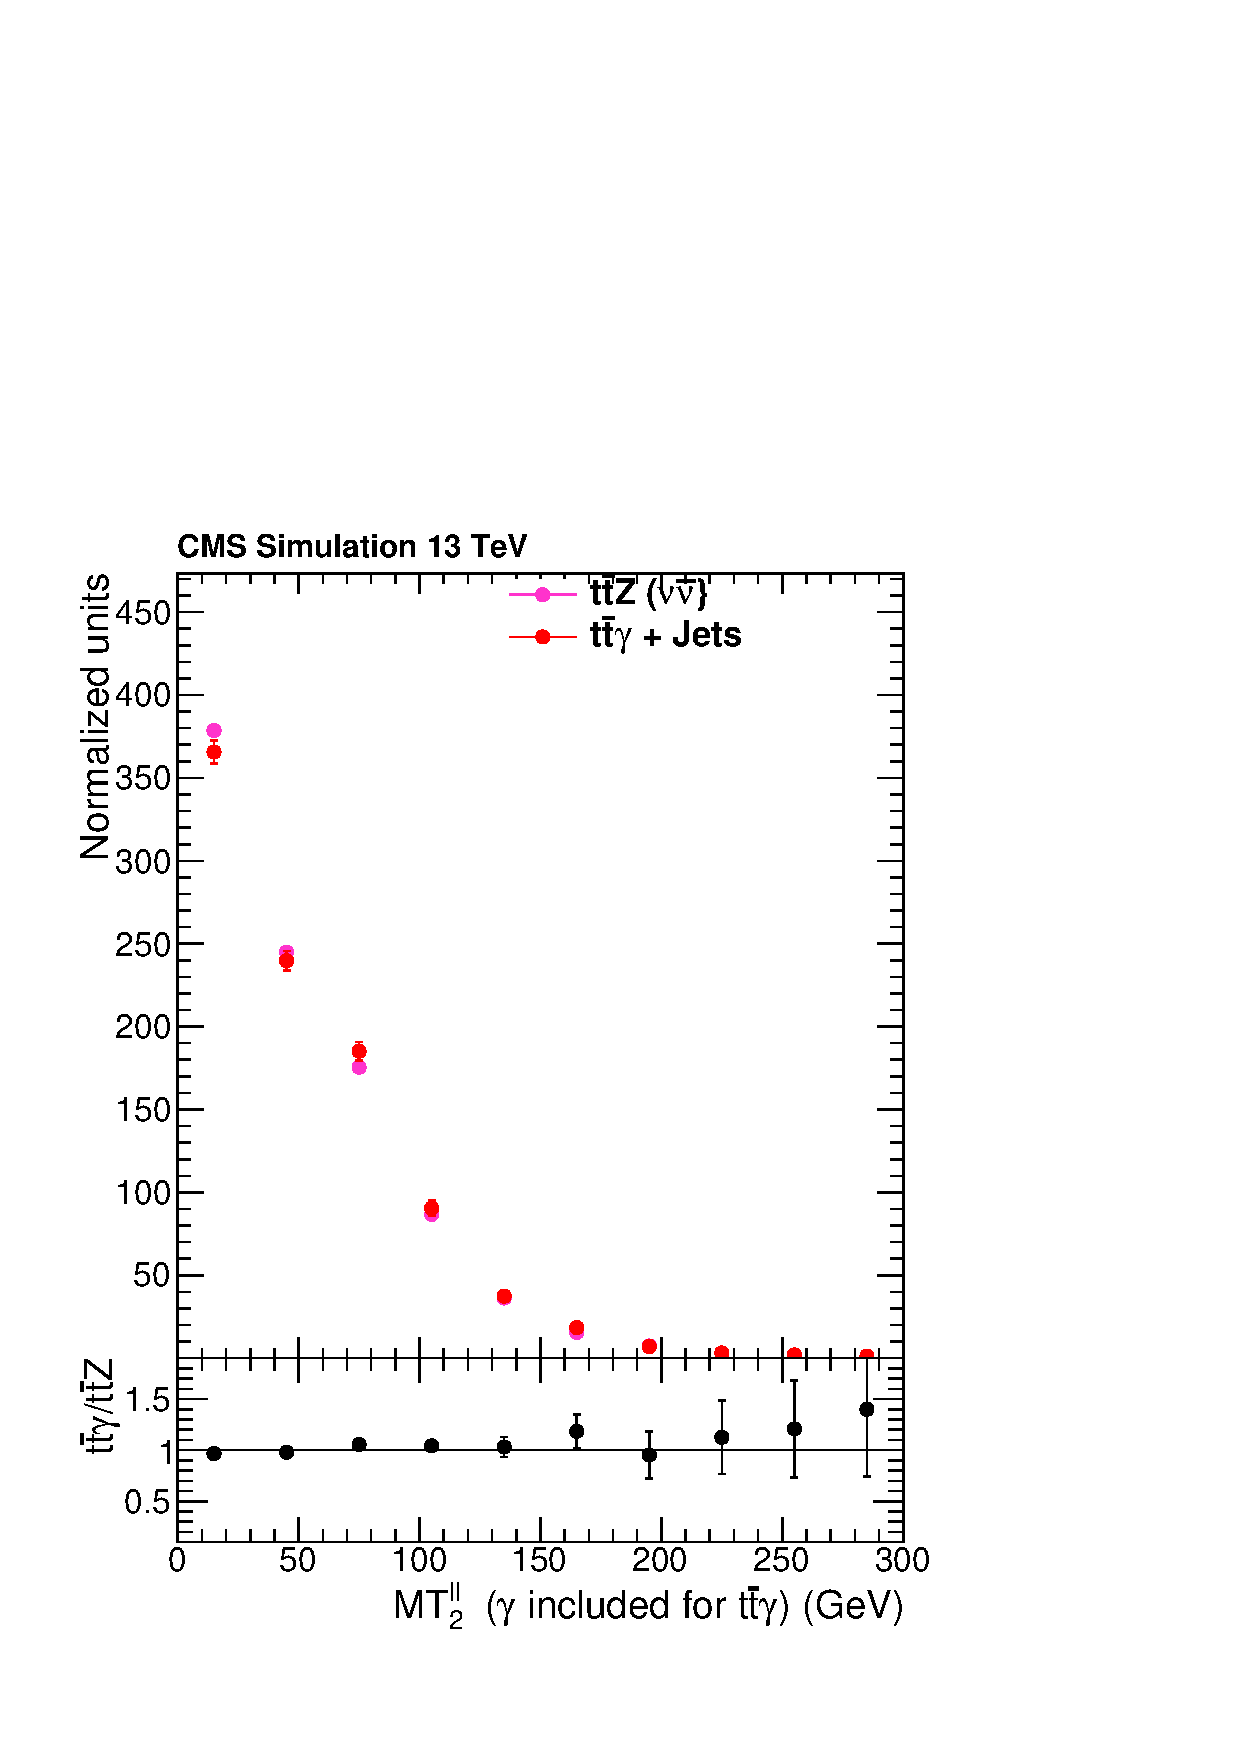
\includegraphics[width=0.45\textwidth]{figures/TTG_gen/reweighted/all_normalized/etaGamma25-ptGamma30/mt2ll_photonIncluded.pdf}}\\
      \subfloat[]{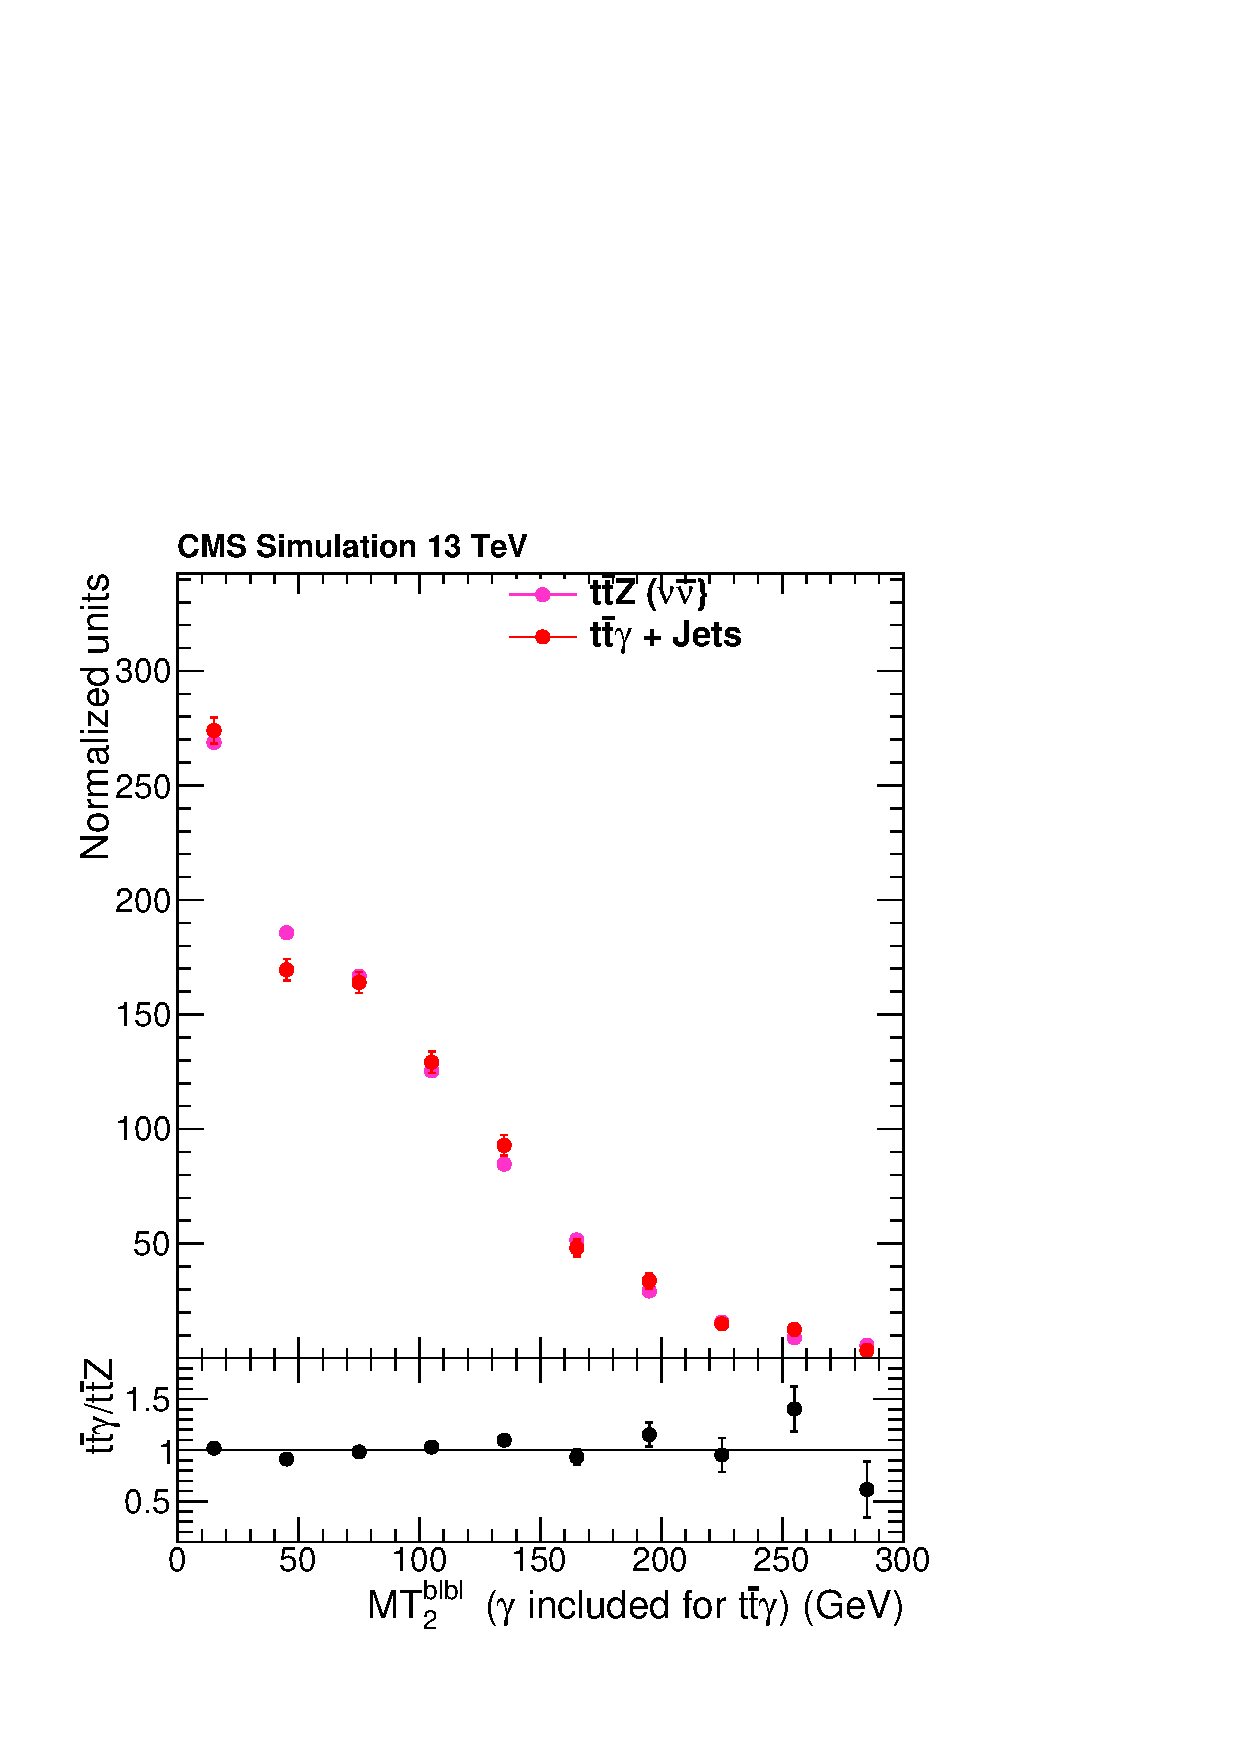
\includegraphics[width=0.45\textwidth]{figures/TTG_gen/reweighted/all_normalized/etaGamma25-ptGamma30/mt2blbl_photonIncluded.pdf}}
      \subfloat[]{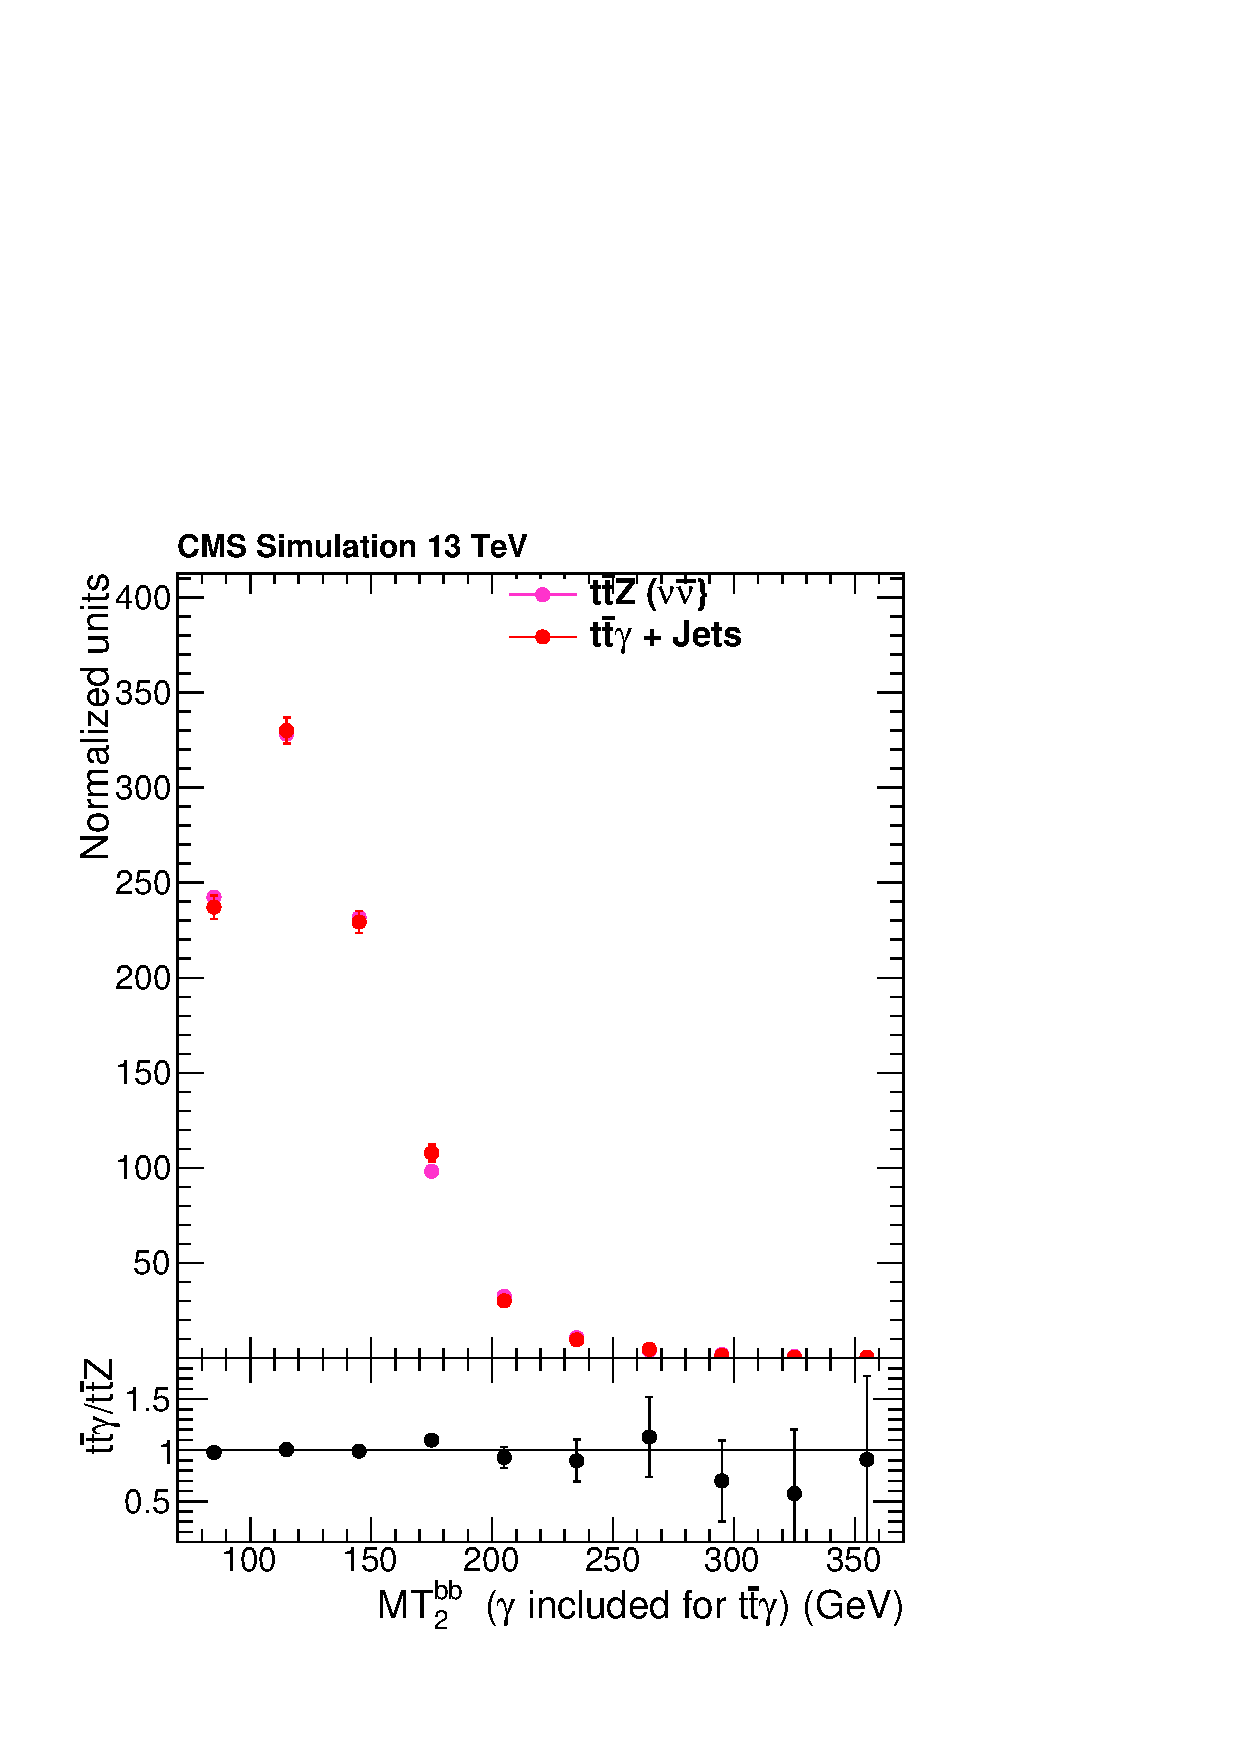
\includegraphics[width=0.45\textwidth]{figures/TTG_gen/reweighted/all_normalized/etaGamma25-ptGamma30/mt2bb_photonIncluded.pdf}}
      \caption{Generator-level comparison of $t\bar{t}\gamma$ (with photon treated as additional \met) with $t\bar{t}Z$ for the \met, \mtll, \mtlblb and \mtbb variables}
      \label{fig:ttgGen}
    \end{figure}

    In order to select a pure $t\bar{t}\gamma$ sample which is closely related to the control and signal regions of our main analysis, we use similar selections but add a photon with $\pt > 30$ \GeV falling within $|\eta| < 2.5$.
    The missing energy cuts are now replaced by \metPhoton and \metSigPhoton which are the photon-estimated variants of \met and \metSig. In order to reduce contributions of $Z\gamma$ events, the $Z$-mass window cut
    is also applied on the invariant mass $m(ll\gamma)$ of the dilepton plus gamma system, as illustrated in Figure~\ref{fig:llg}. Furthermore, photons are required to have $\Delta R(\gamma, l) > 0.3$ and $\Delta R(\gamma, j) > 0.3$, of which the latter
    is used to reject photons which are constructed as jets.
    \begin{table}
  \center
  \small
  \begin{tabular}{c|c}
                     & photons         \\
     \hline
     \pt             & $> 30\GeV$    \\    
     $|\eta|$        & $< 2.5$         \\   
     identification  & cut-based tight id  \\
  \end{tabular}
  \caption{Photon selection criteria}
  \label{photonSelection}
\end{table}


    Figure~\ref{fig:ttg_met} shows the \metPhoton before requiring the $\metPhoton > 80 \GeV$ requirement and \metSigPhoton before requiring $\metSigPhoton > 5$. The distributions of
    the photon-estimated \mtll, \mtlblb and \mtbb variables before applying the \met and \metSigPhoton requirements is shown in Figure~\ref{fig:ttg_mt2}.
    Figures~\ref{fig:ttg_mt2ll},~\ref{fig:ttg_mt2blbl} and~\ref{fig:ttg_mt2bb} show these variables after \met, \metSig and $\Delta\phi(\met, j)$ cuts, both before and after subtraction of the residual backgrounds.
    Based on the level of agreement we assign a 20\% uncertainty from the \mtll shape of TTZ. 
    
    % Data plots
    \begin{figure}
      \centering
      \subfloat[before $m(ll\gamma)$ cut]{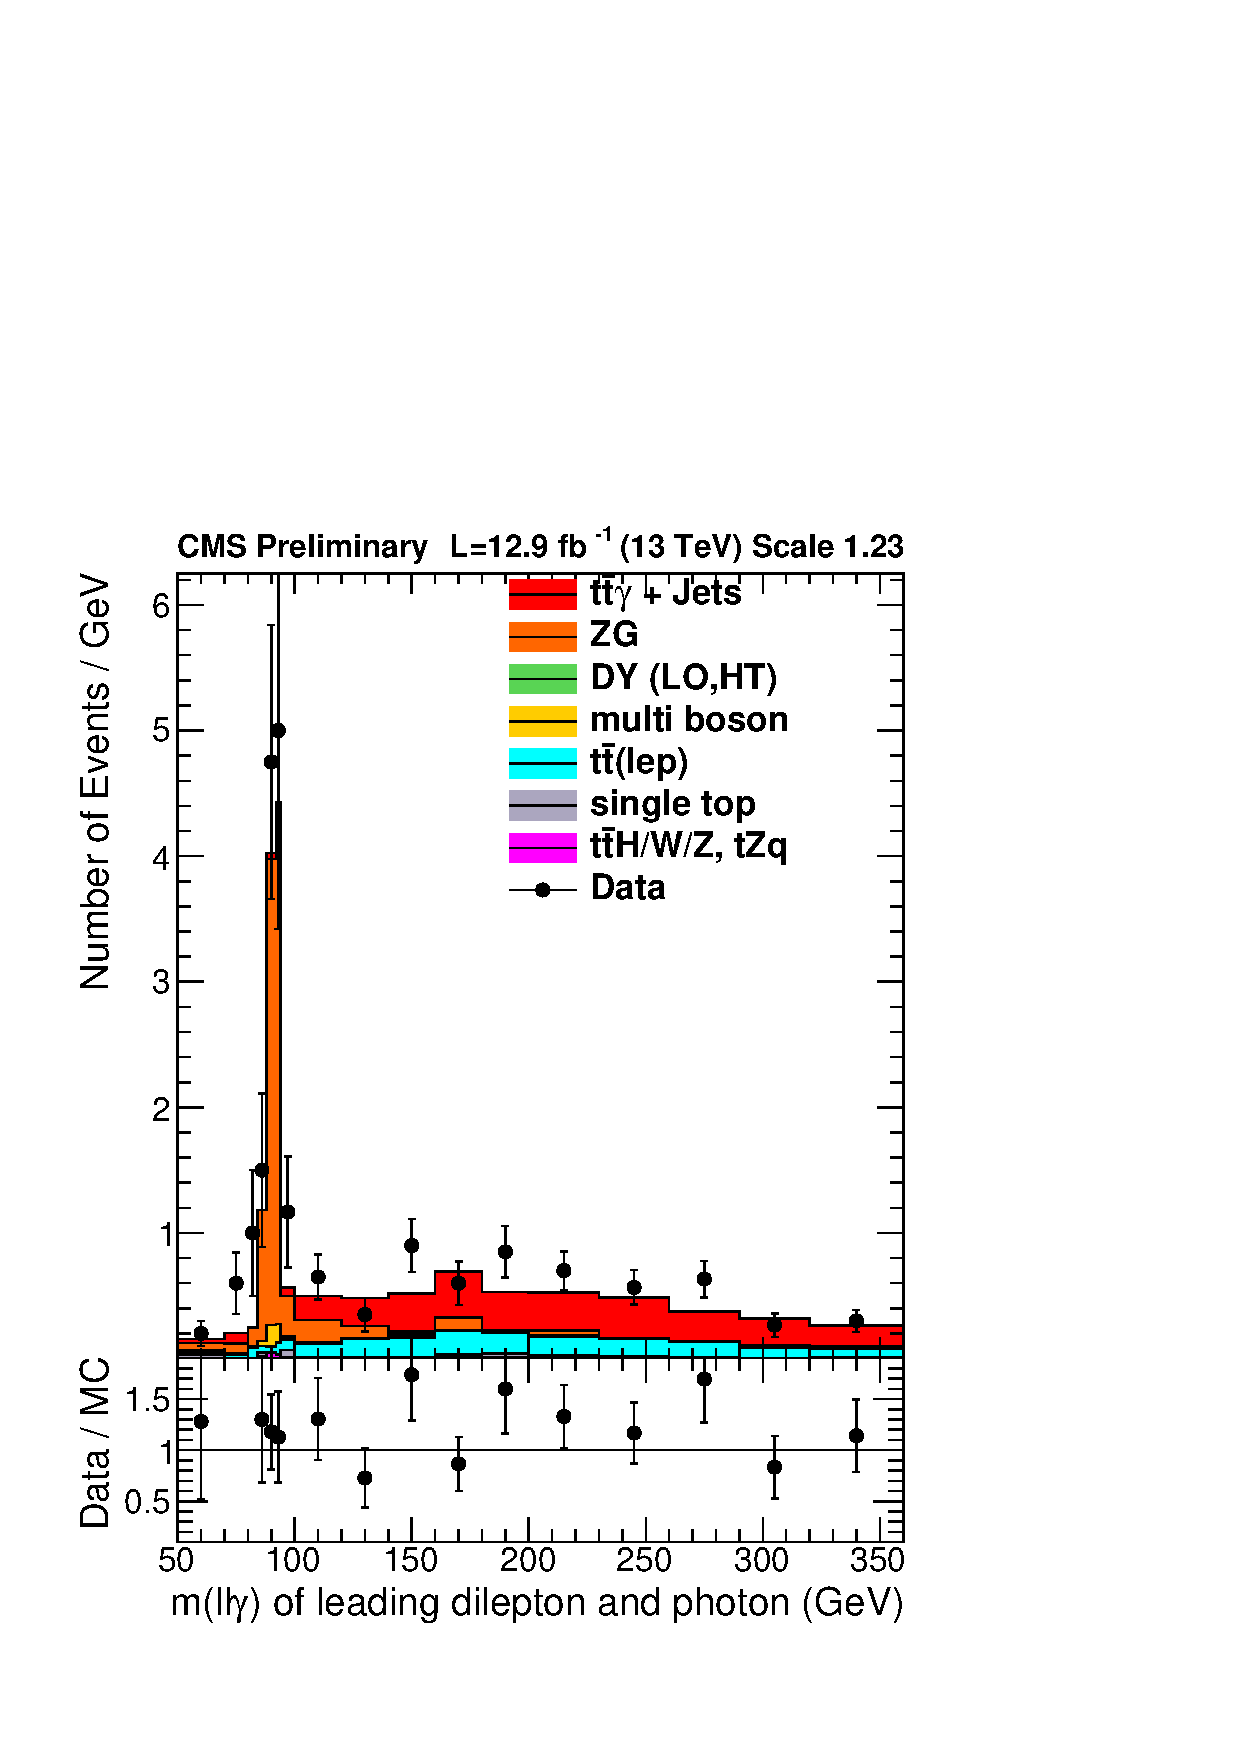
\includegraphics[width=0.45\textwidth]{figures/TTG/all/njet2-photon30-gJetdR-gLepdR-btagM/dlg_mass.pdf}}
      \subfloat[after $m(ll\gamma)$ cut]{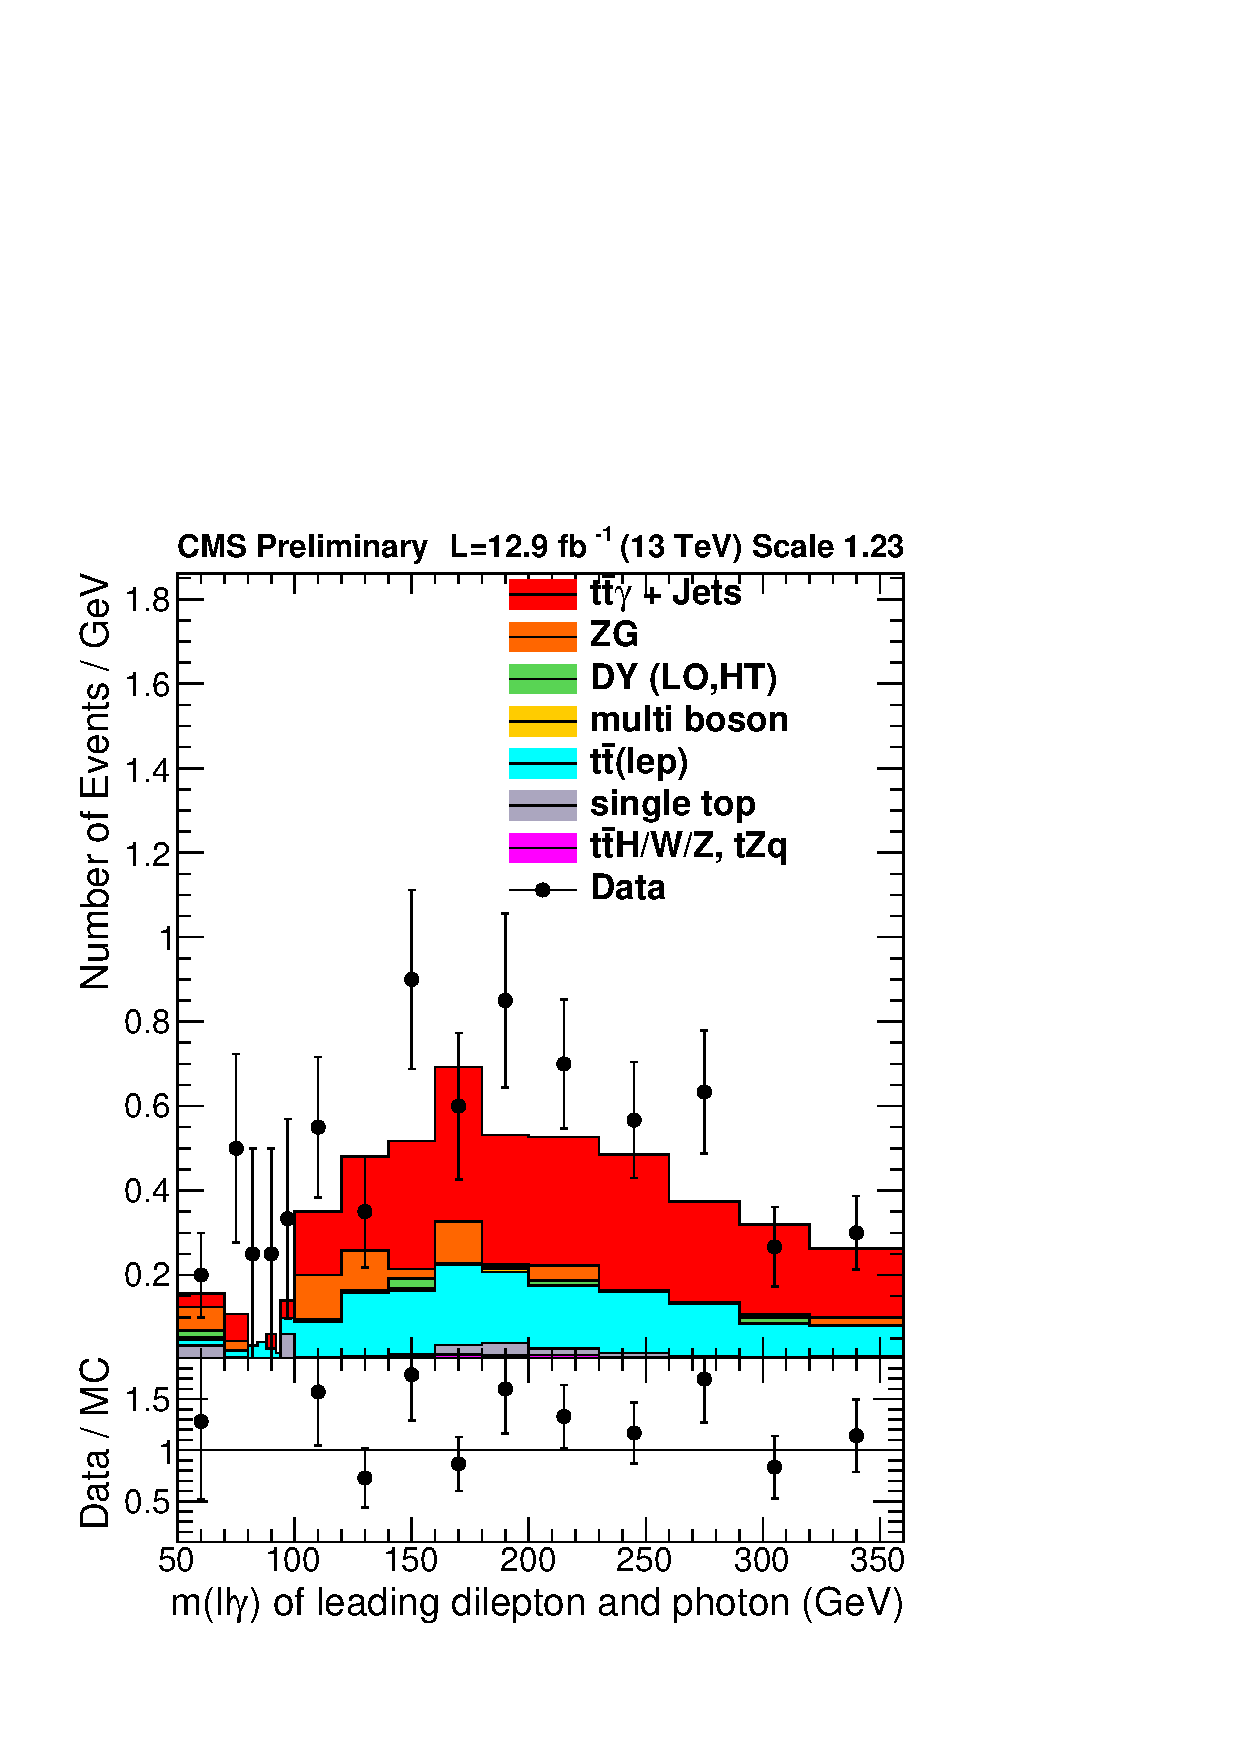
\includegraphics[width=0.45\textwidth]{figures/TTG/all/njet2-photon30-llgNoZ-gJetdR-gLepdR-btagM/dlg_mass.pdf}}
      \caption{Requiring a $Z$ window on $m(ll\gamma)$ in the same-flavour channels removes most of the $Z\gamma$ background. Given the sharp $Z$ peak in combination with a low-statistics tail, a dynamic binning
      is used for these plots, each bin showing the average number of events per \GeV for its $m(ll\gamma)$ range.}
      \label{fig:llg}
    \end{figure}

    \begin{figure}
      \centering
      \subfloat[\metPhoton]{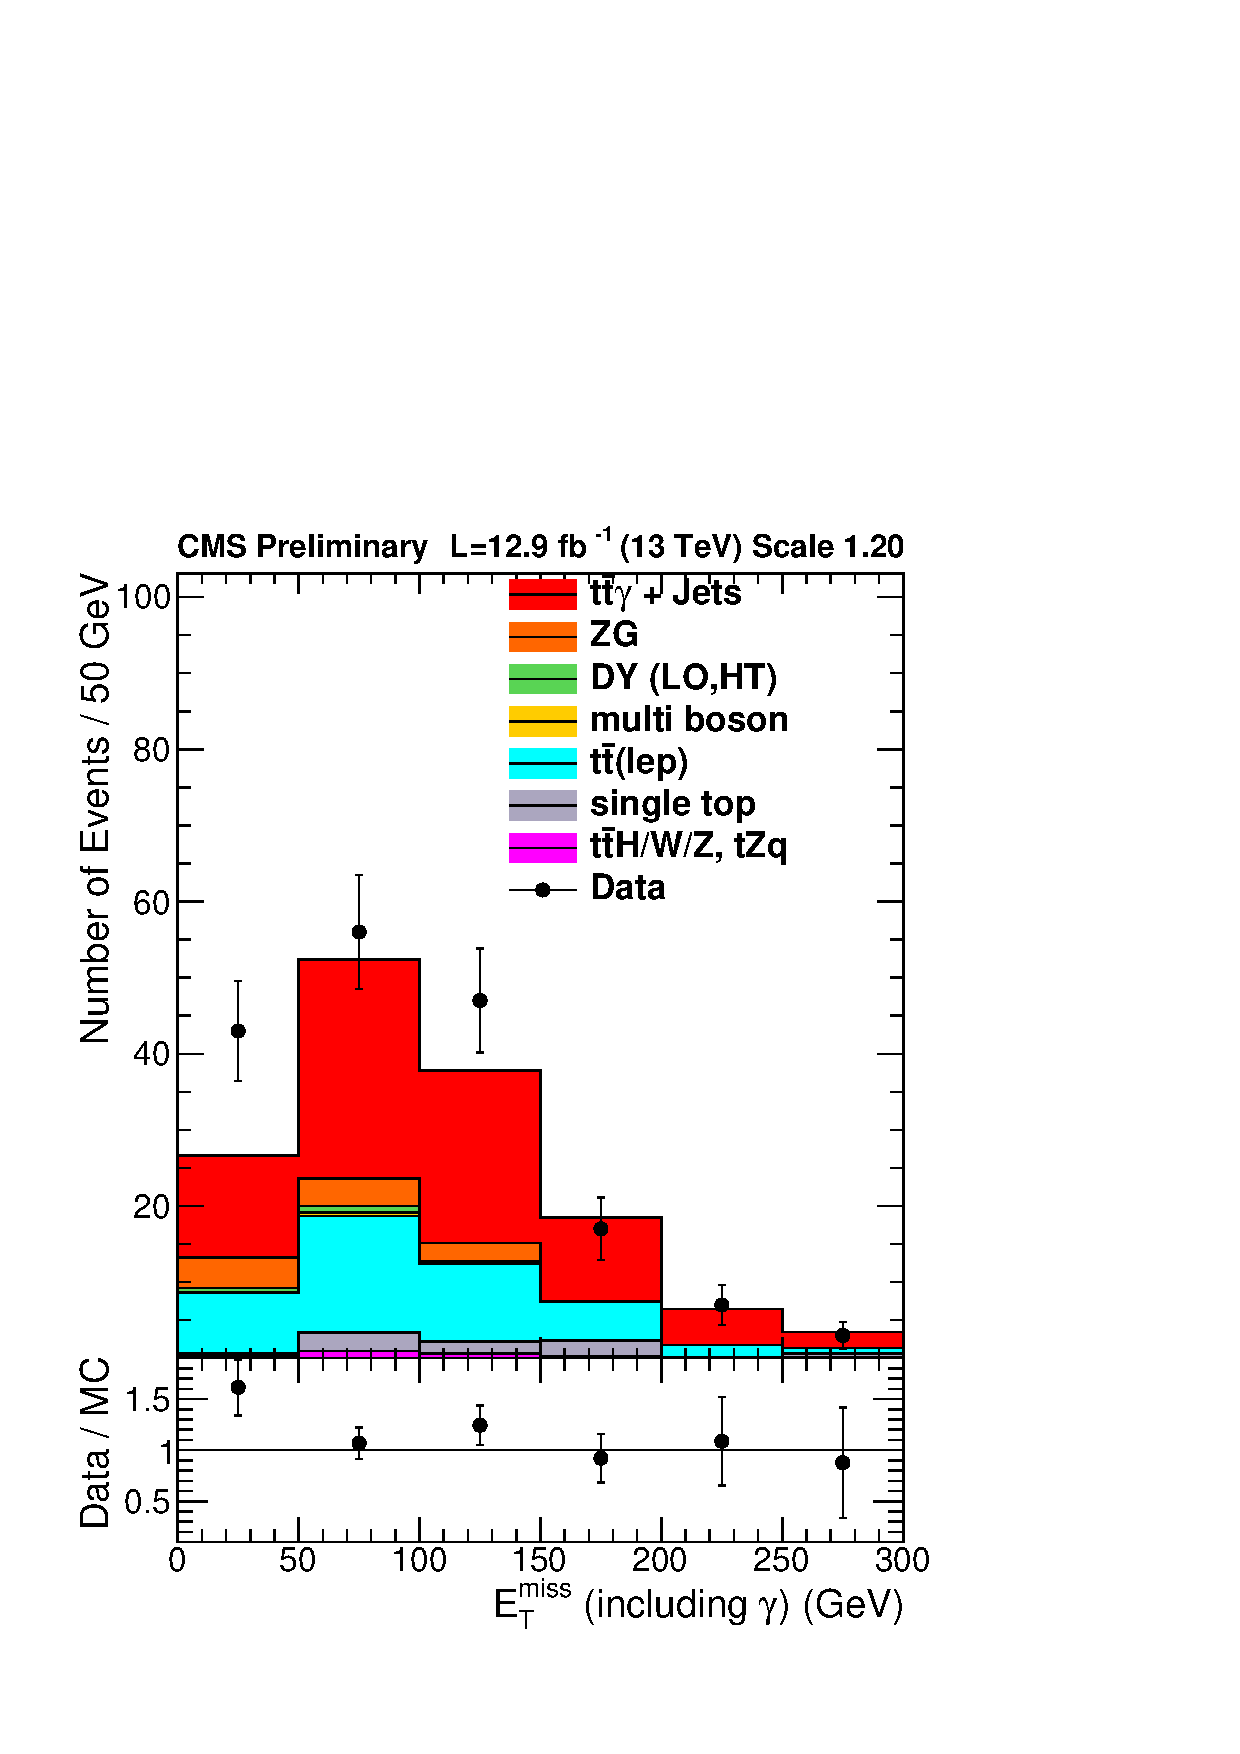
\includegraphics[width=0.45\textwidth]{figures/TTG/all/njet2-photon30-llgNoZ-gJetdR-gLepdR-btagM-mll20/met_pt_photonEstimated.pdf}}
      \subfloat[\metSigPhoton]{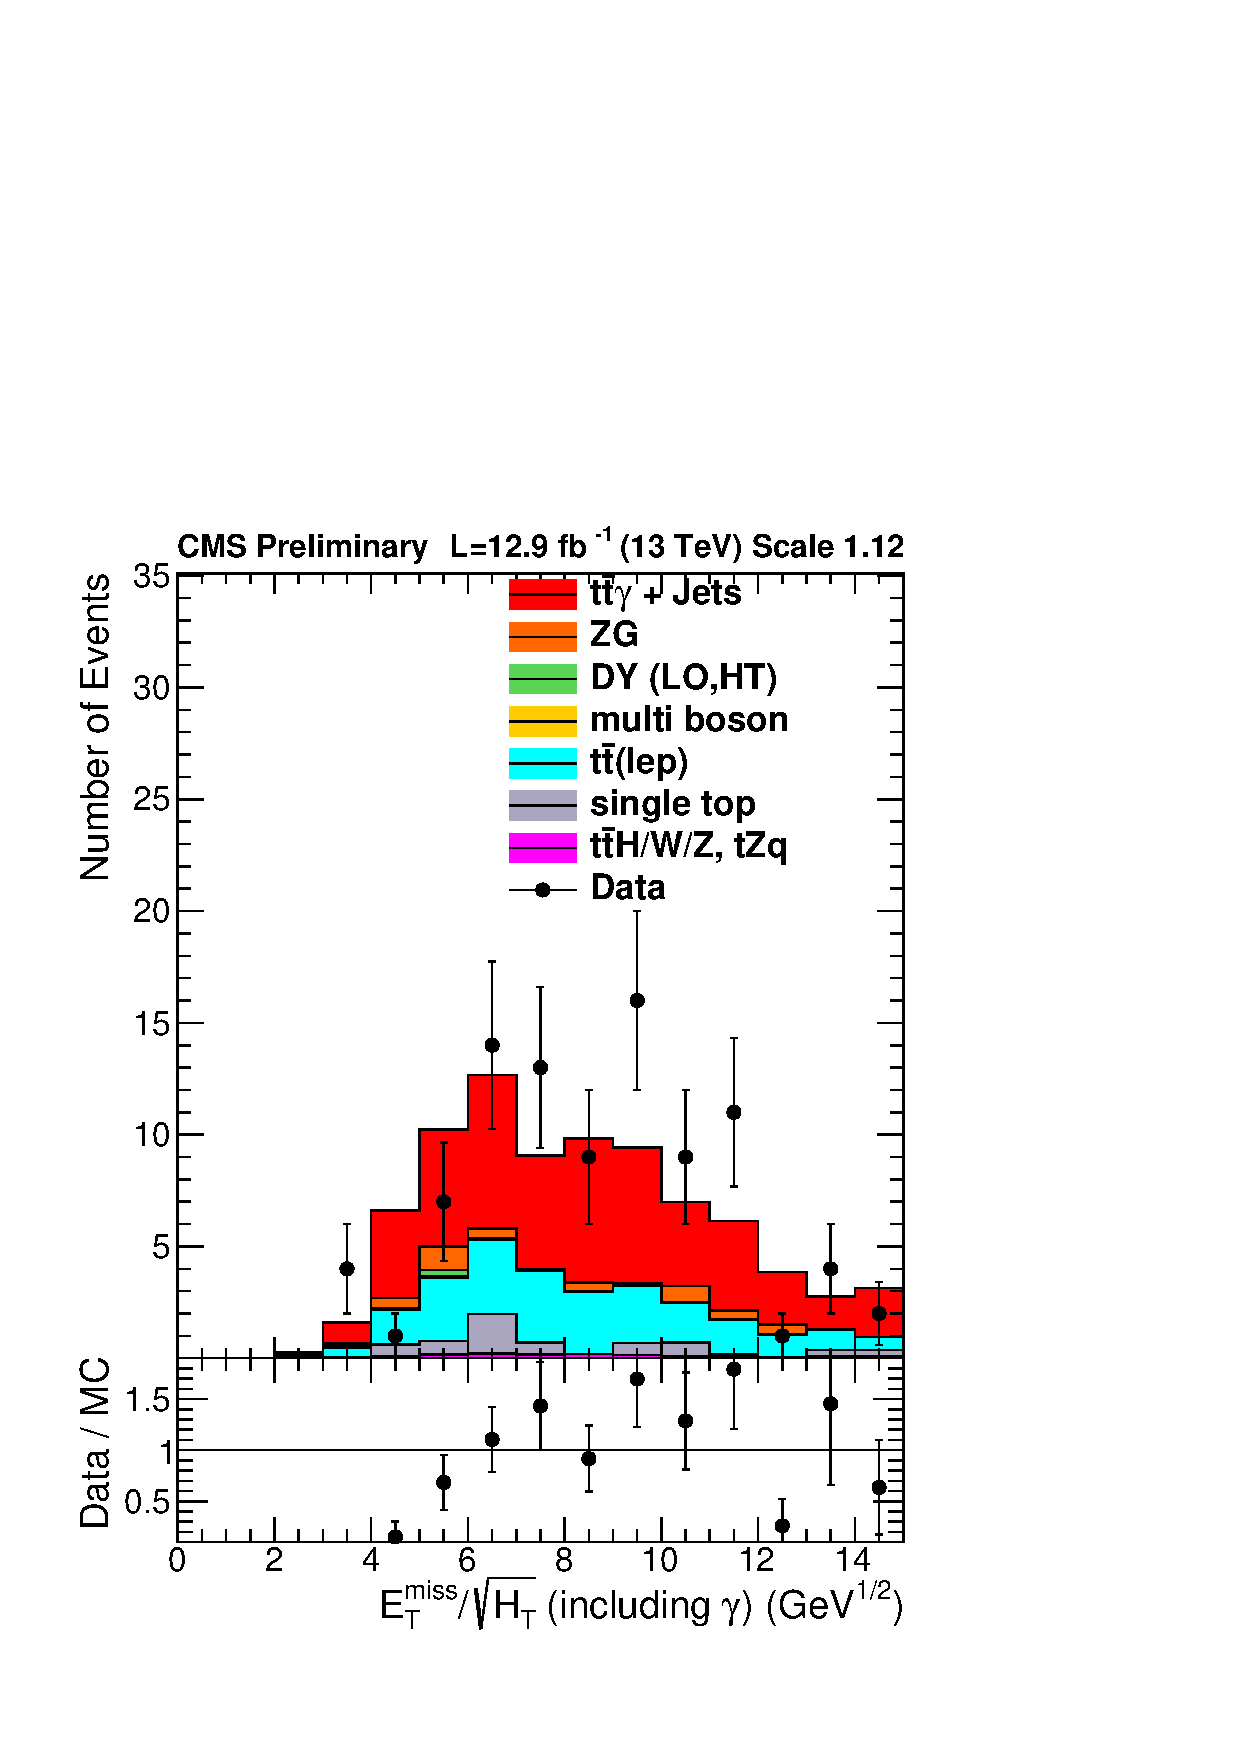
\includegraphics[width=0.45\textwidth]{figures/TTG/all/njet2-photon30-llgNoZ-gJetdR-gLepdR-btagM-mll20-met80/metSig_photonEstimated.pdf}}
      \caption{Distribution of \metPhoton and \metSigPhoton with photon \pt included in the \met calculation, before cutting on them}
      \label{fig:ttg_met}
    \end{figure}

    \begin{figure}
      \centering
      \subfloat[\mtll]{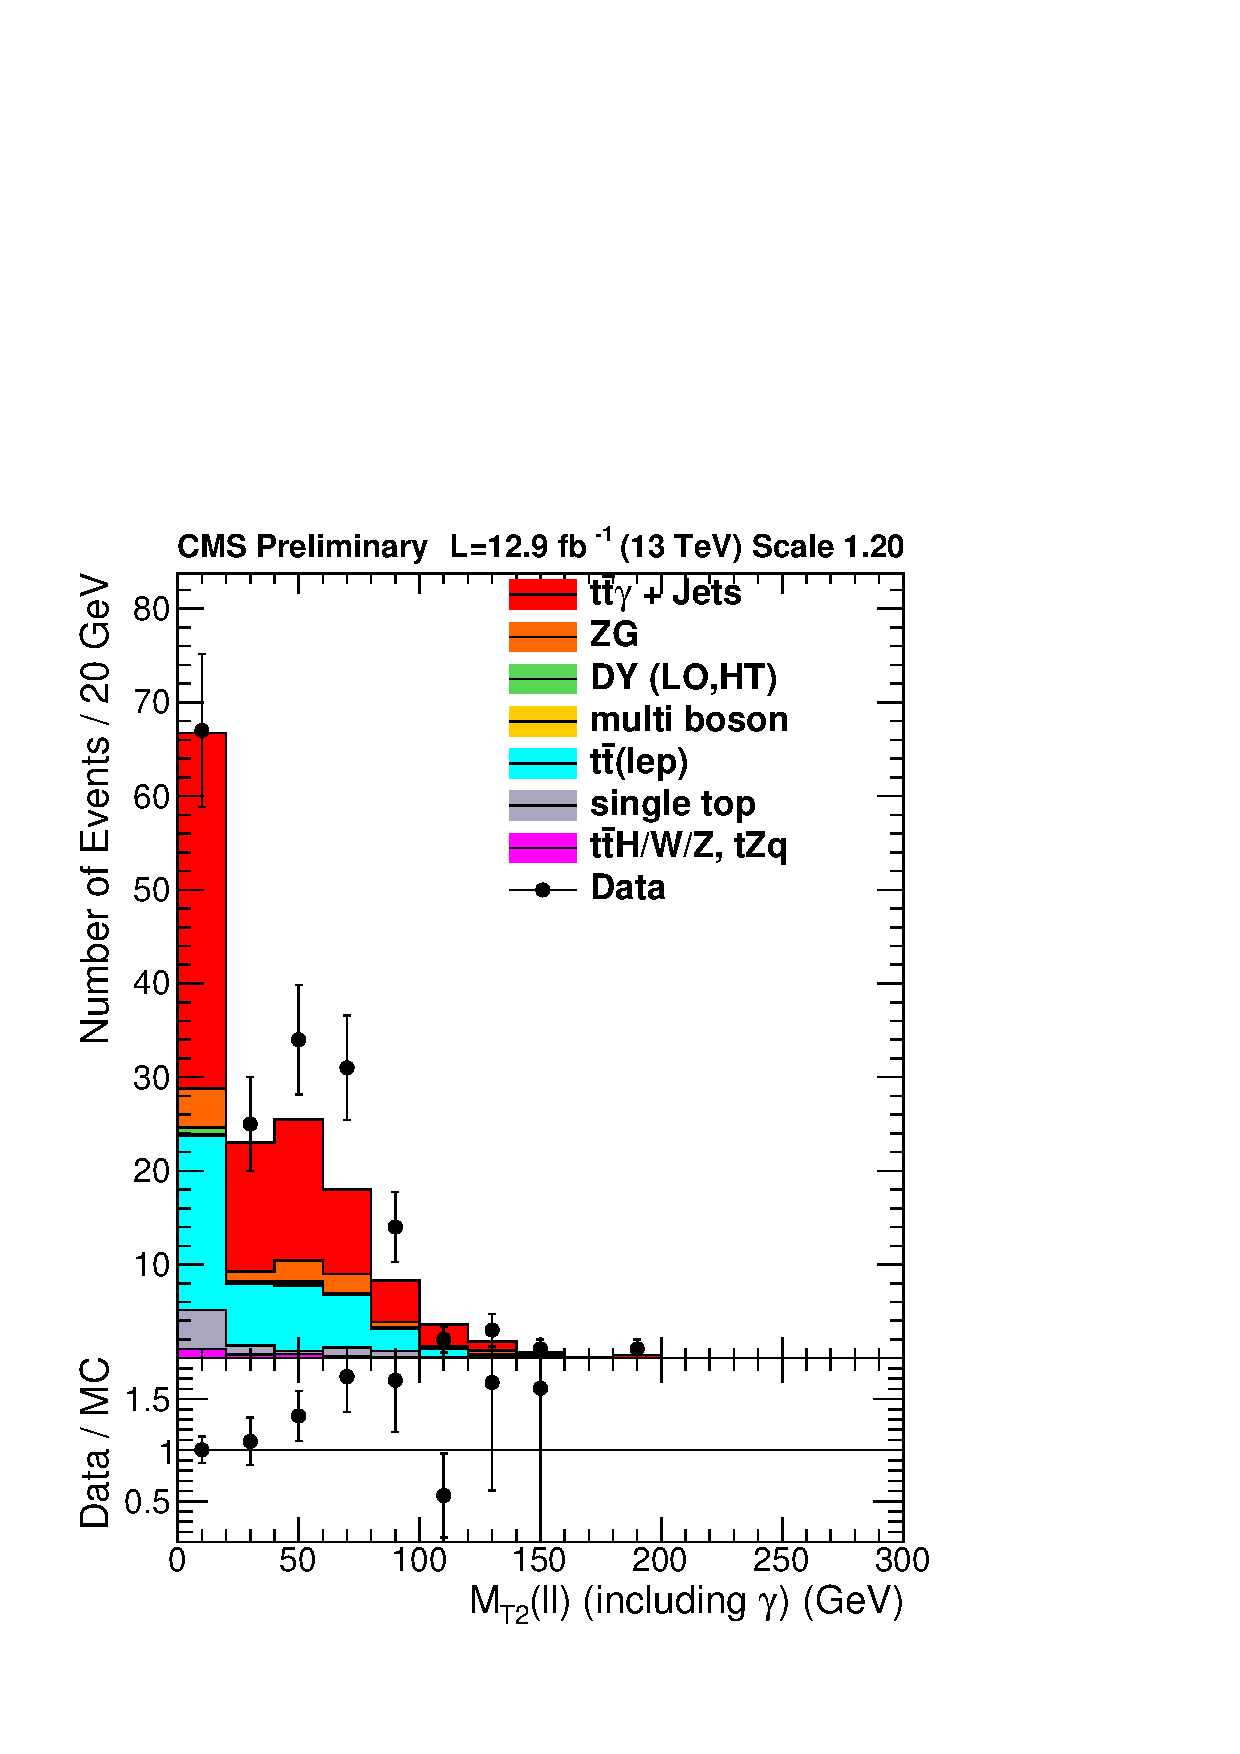
\includegraphics[width=0.32\textwidth]{figures/TTG/all/njet2-photon30-llgNoZ-gJetdR-gLepdR-btagM-mll20/dl_mt2ll_photonEstimated.pdf}}
      \subfloat[\mtlblb]{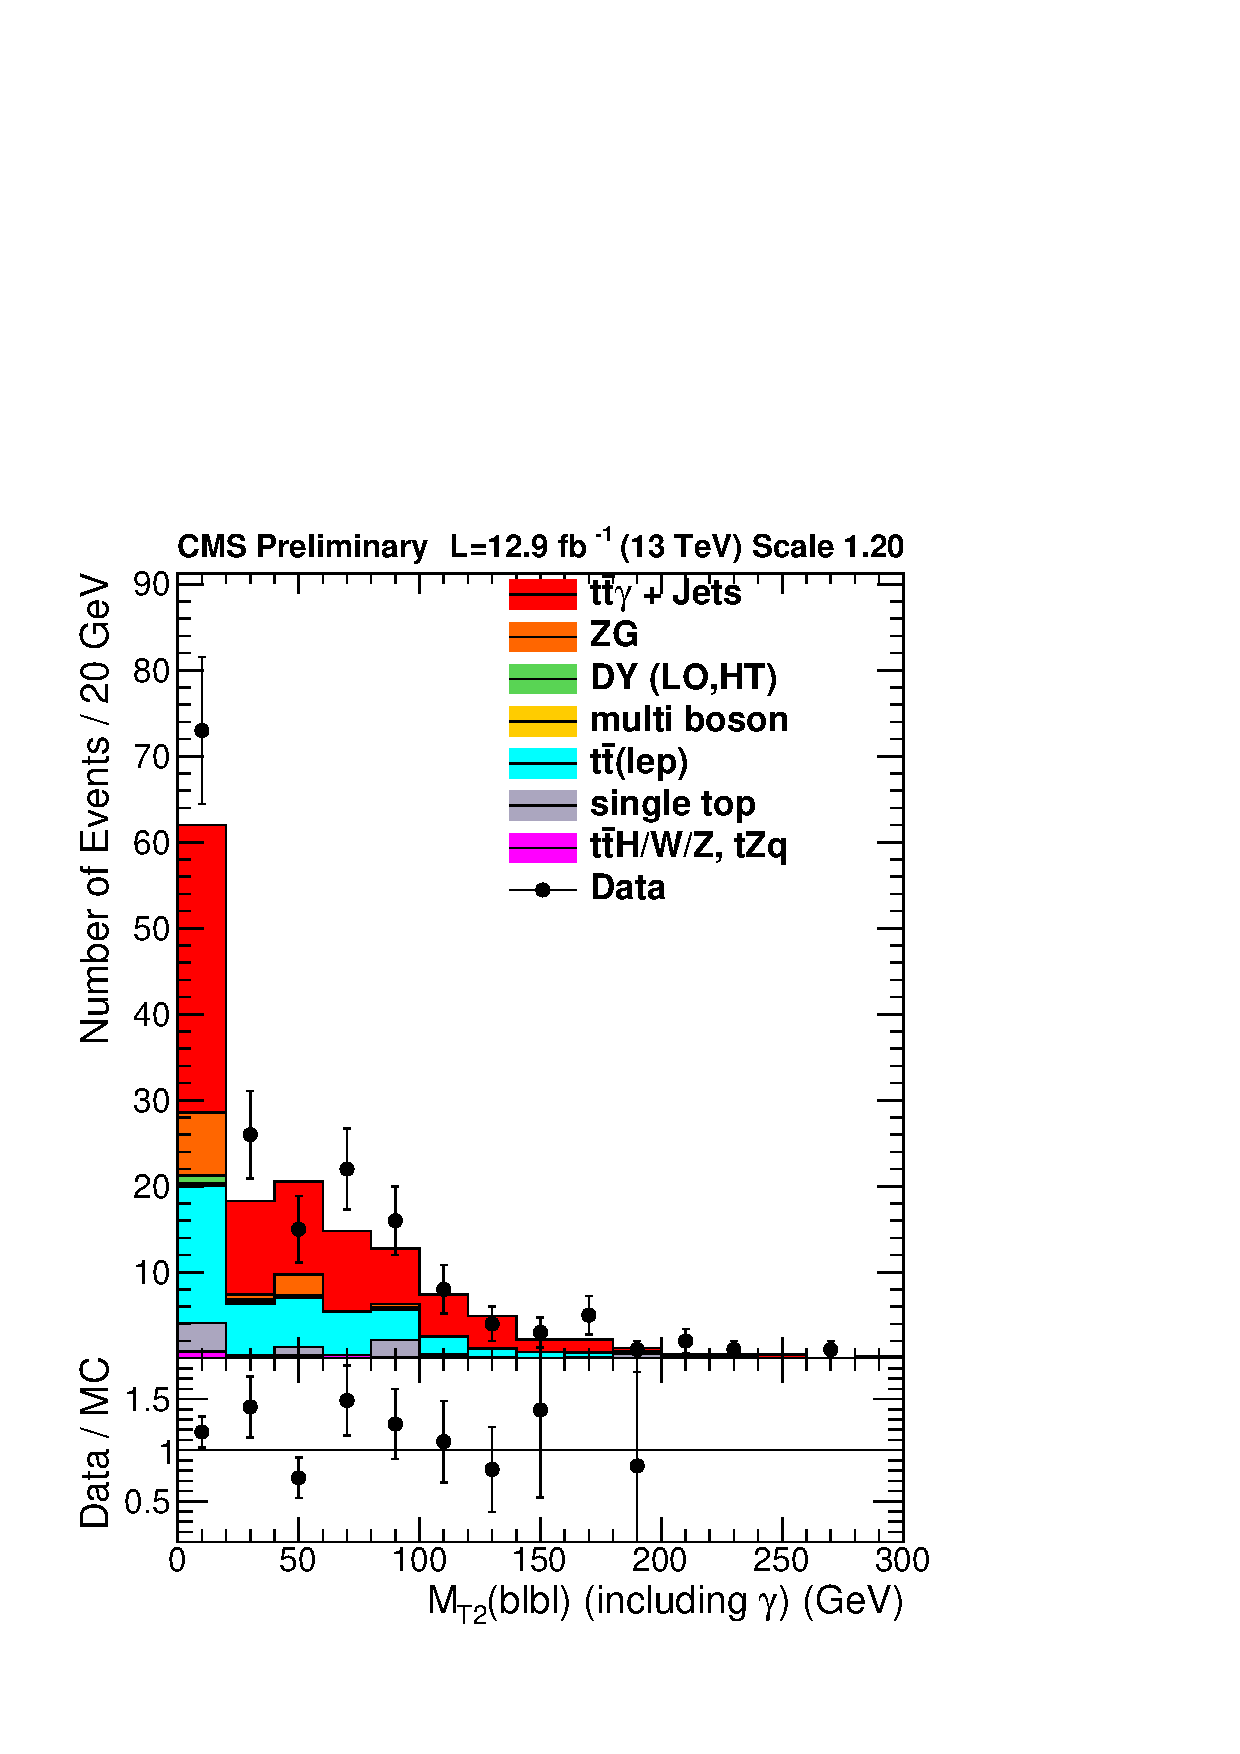
\includegraphics[width=0.32\textwidth]{figures/TTG/all/njet2-photon30-llgNoZ-gJetdR-gLepdR-btagM-mll20/dl_mt2blbl_photonEstimated.pdf}}
      \subfloat[\mtbb]{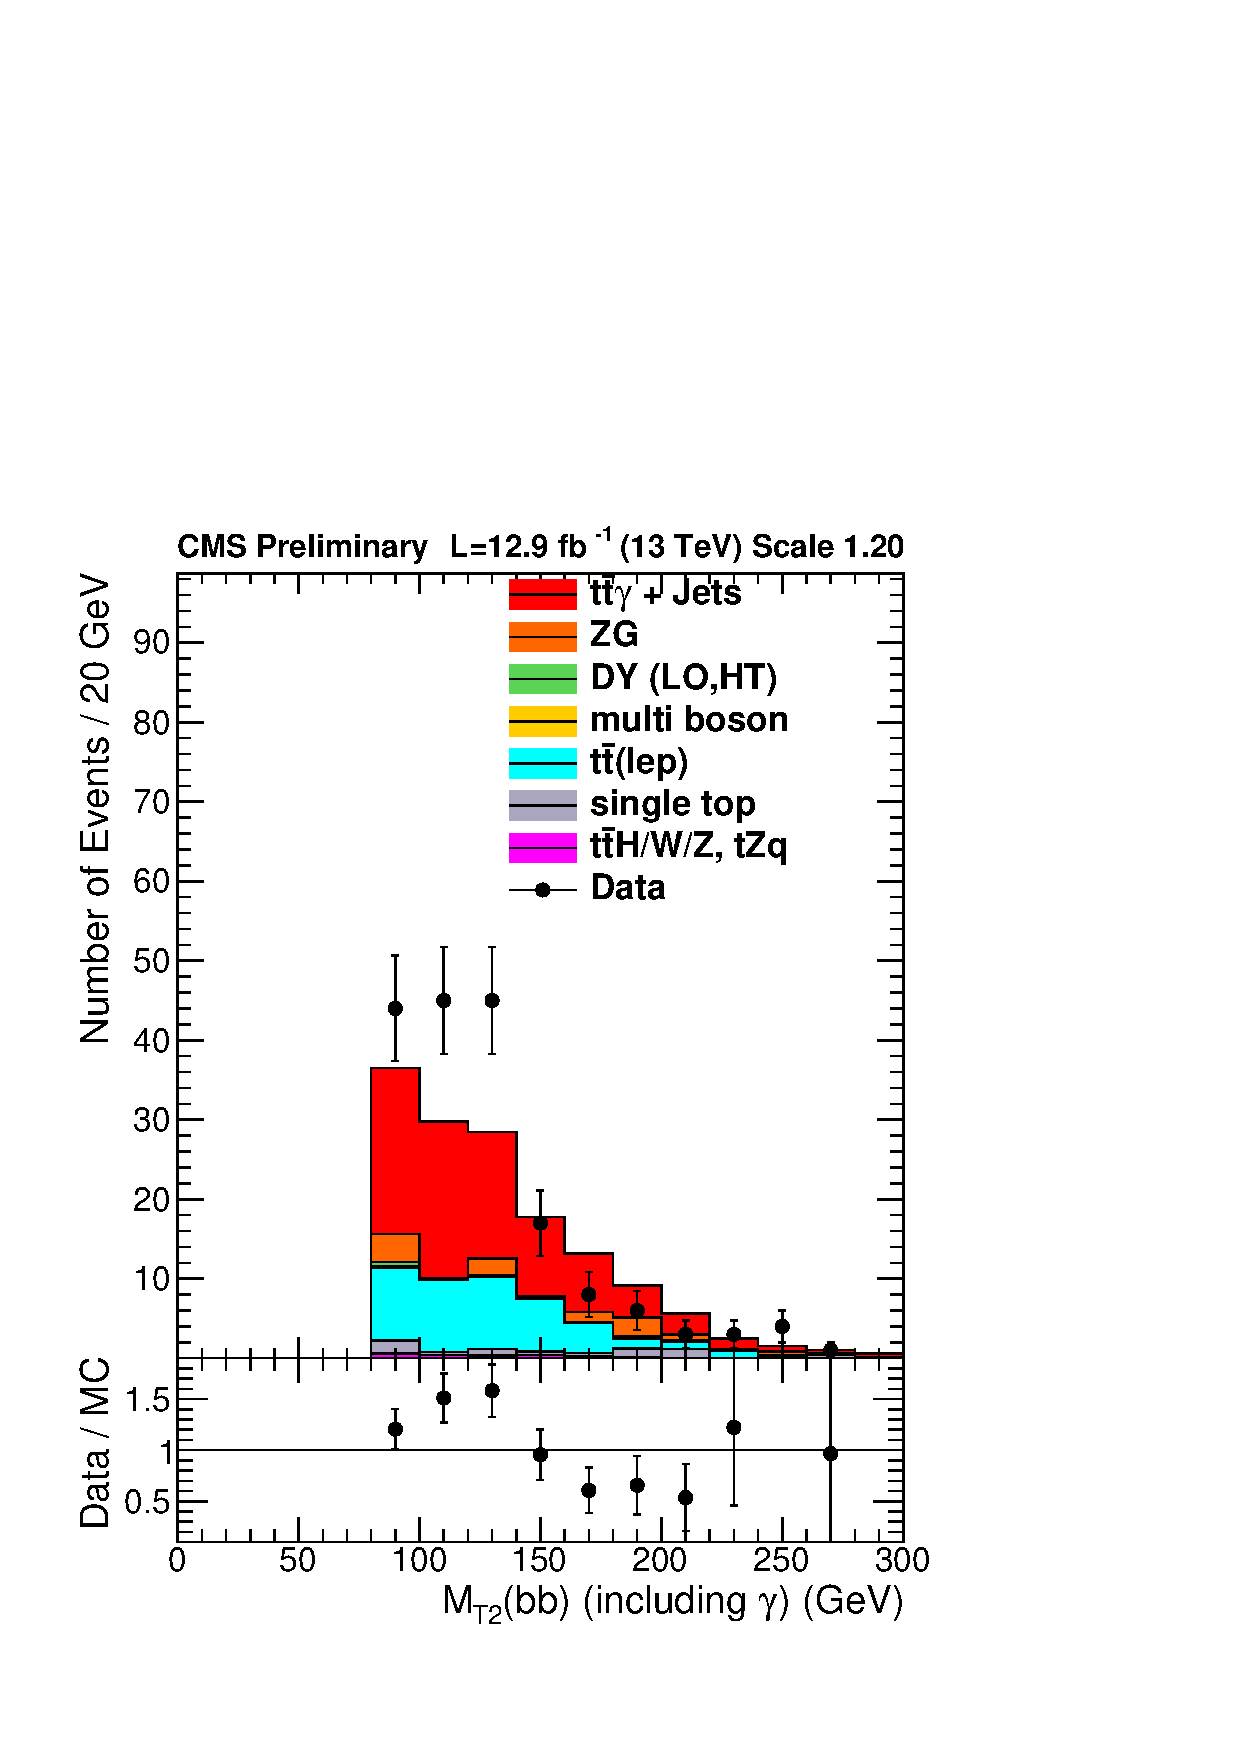
\includegraphics[width=0.32\textwidth]{figures/TTG/all/njet2-photon30-llgNoZ-gJetdR-gLepdR-btagM-mll20/dl_mt2bb_photonEstimated.pdf}}
      \caption{Distribution of \mtll, \mtlblb and \mtbb using the photon-estimated \metPhoton}
      \label{fig:ttg_mt2}
    \end{figure}

    \begin{figure}
      \centering
      \subfloat[other MC included]{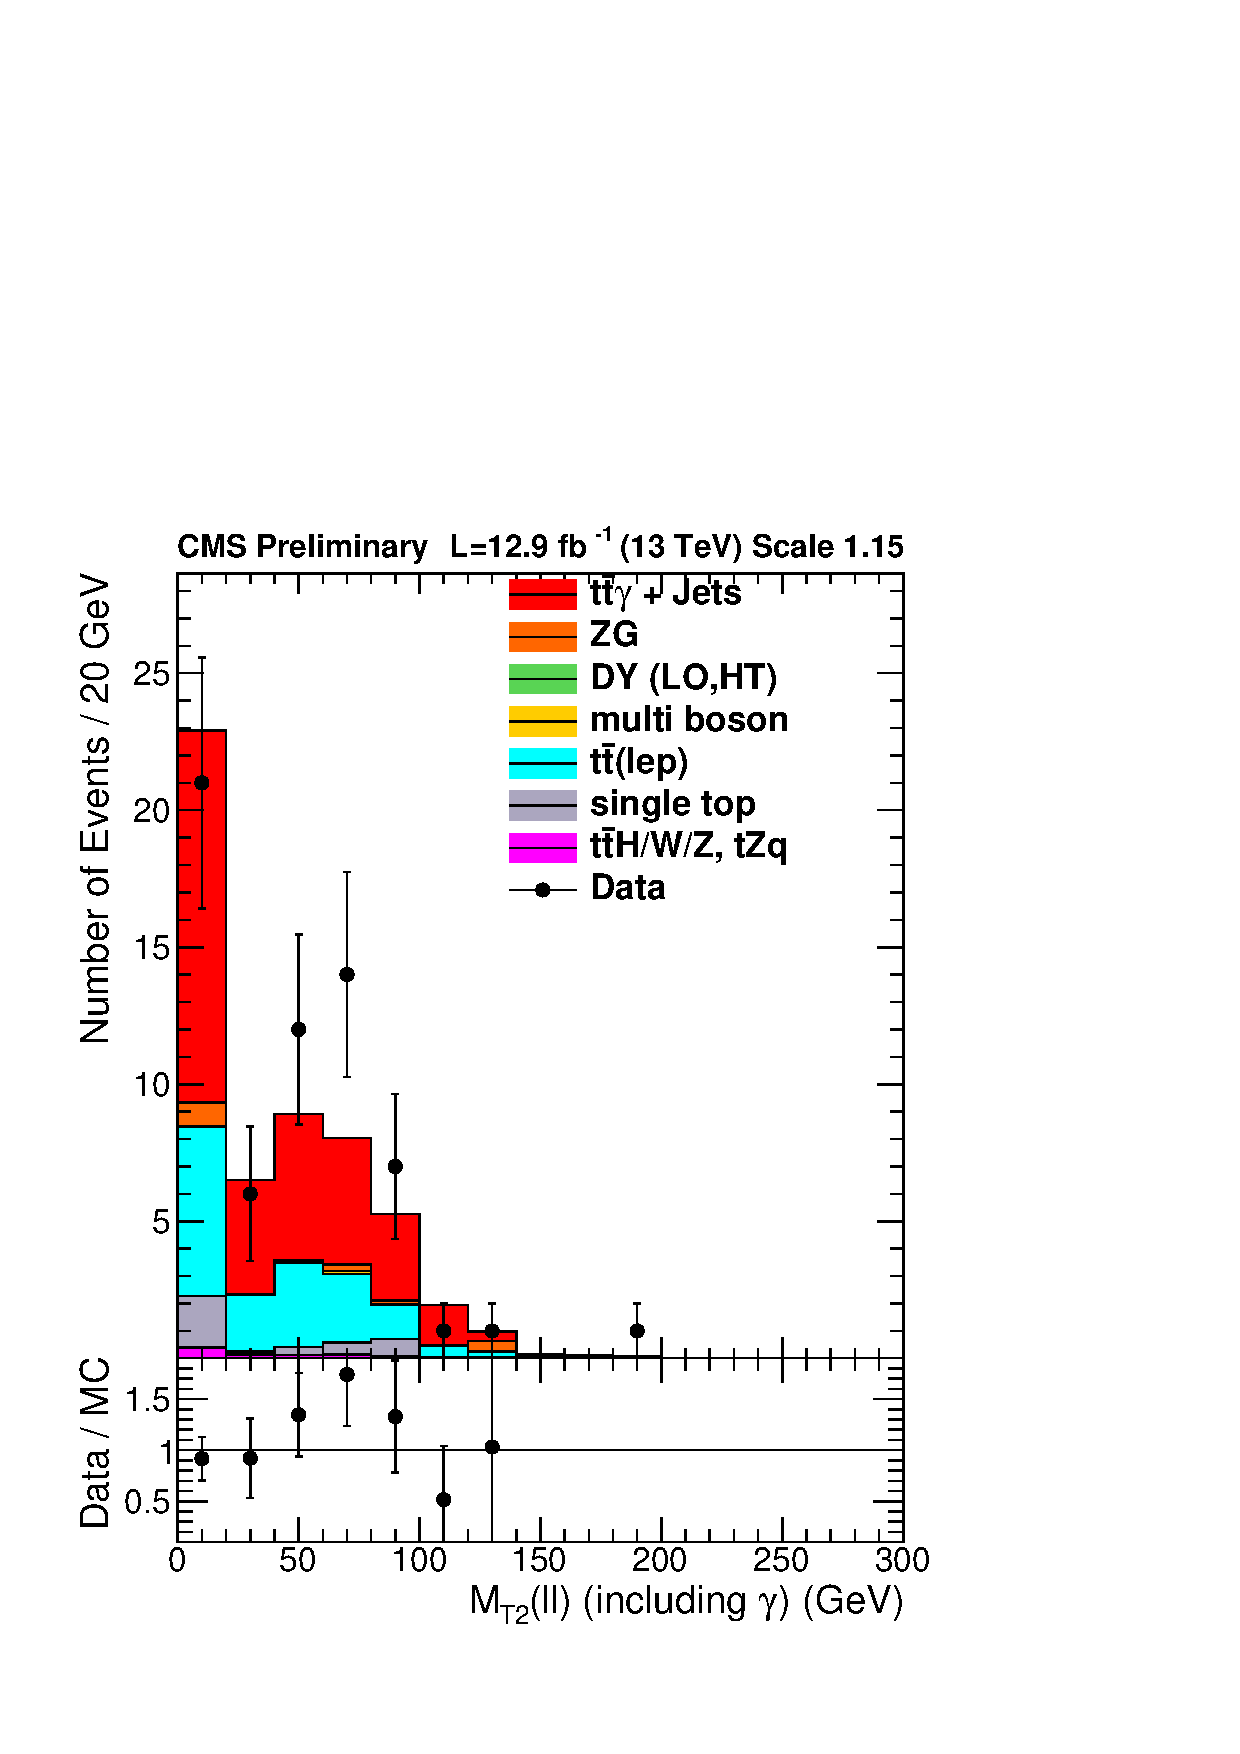
\includegraphics[width=0.45\textwidth]{figures/TTG/all/njet2-photon30-llgNoZ-gJetdR-gLepdR-btagM-mll20-met80-metSig5-dPhiJet0-dPhiJet1/dl_mt2ll_photonEstimated.pdf}}
      \subfloat[other MC subtracted]{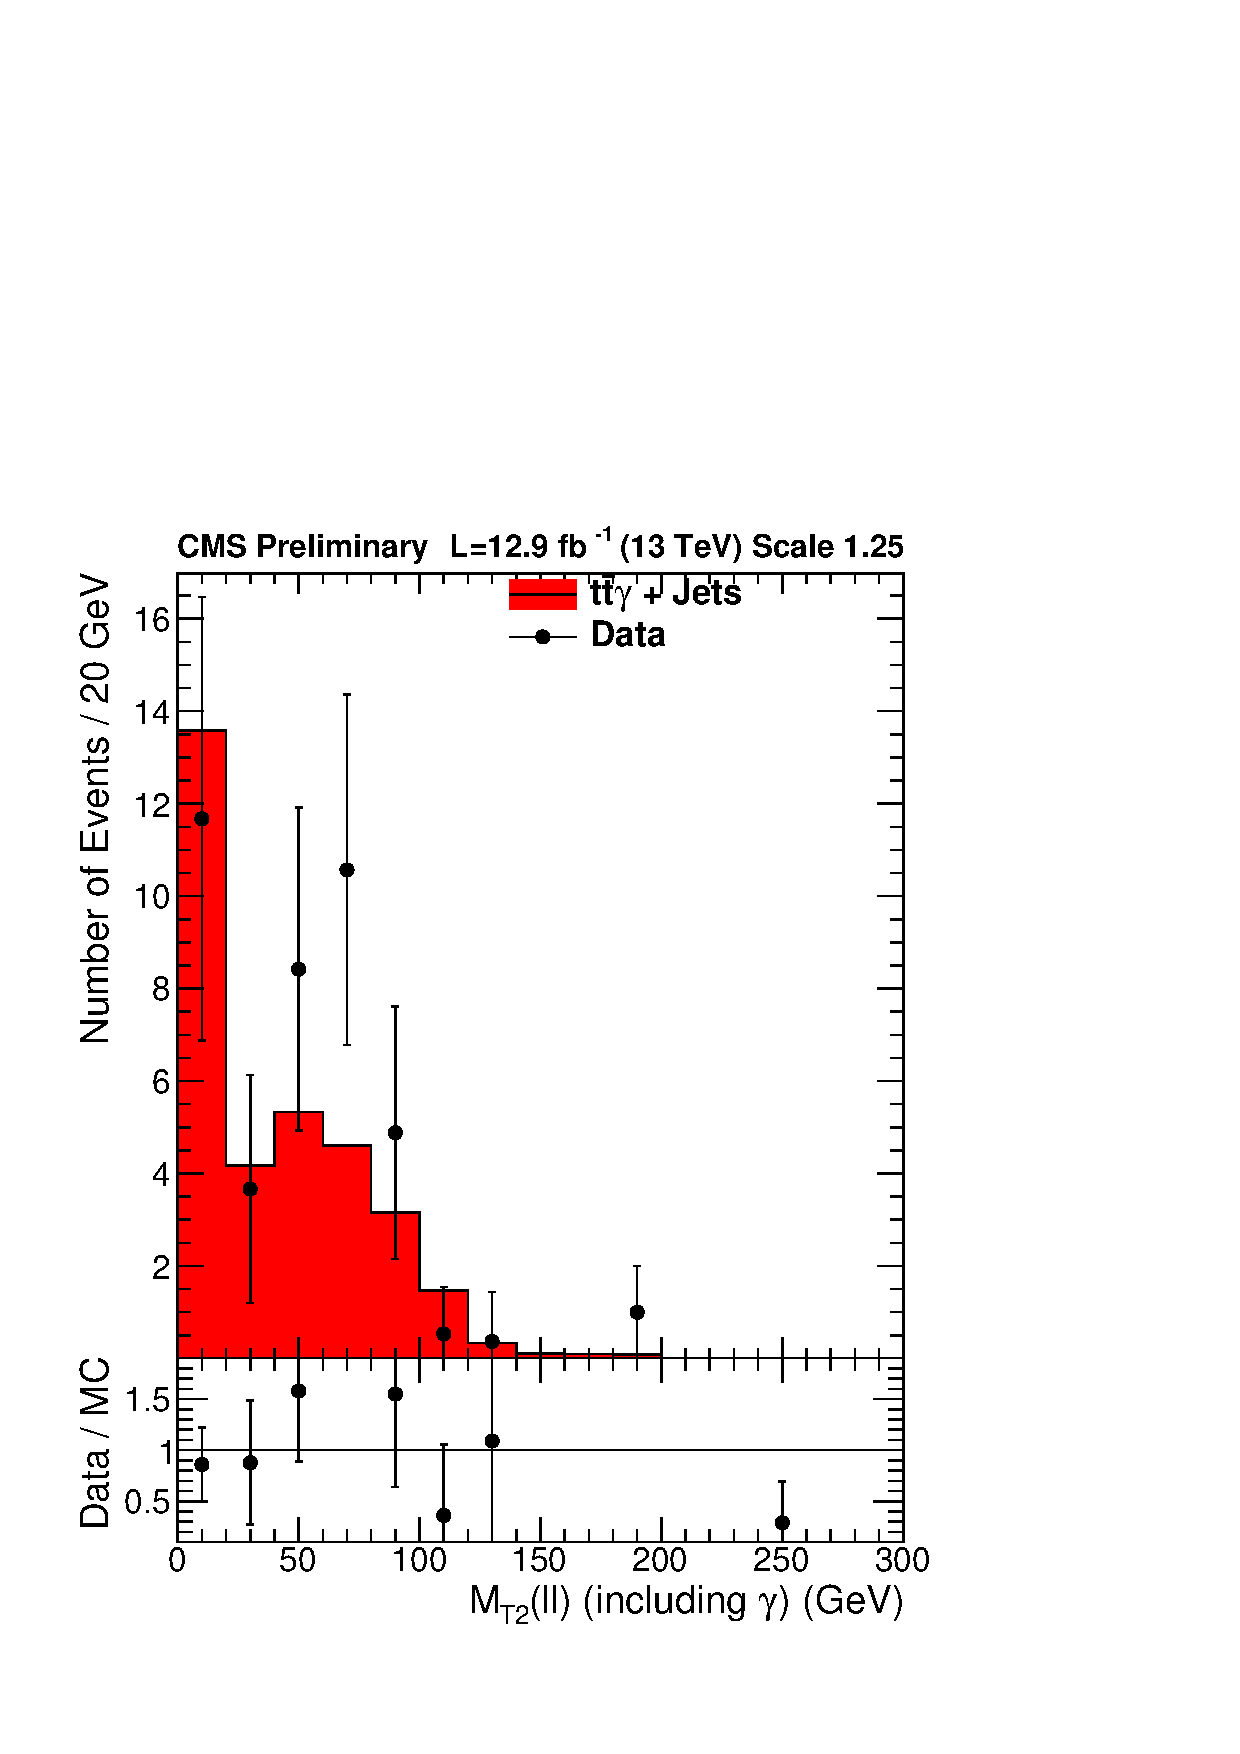
\includegraphics[width=0.45\textwidth]{figures/TTG_subtracted/all/njet2-photon30-llgNoZ-gJetdR-gLepdR-btagM-mll20-met80-metSig5-dPhiJet0-dPhiJet1/dl_mt2ll_photonEstimated.pdf}}
      \caption{Distribution of \mtll using the photon-estimated \metPhoton (after \met cuts)}
      \label{fig:ttg_mt2ll}
    \end{figure}

    \begin{figure}
      \centering
      \subfloat[other MC included]{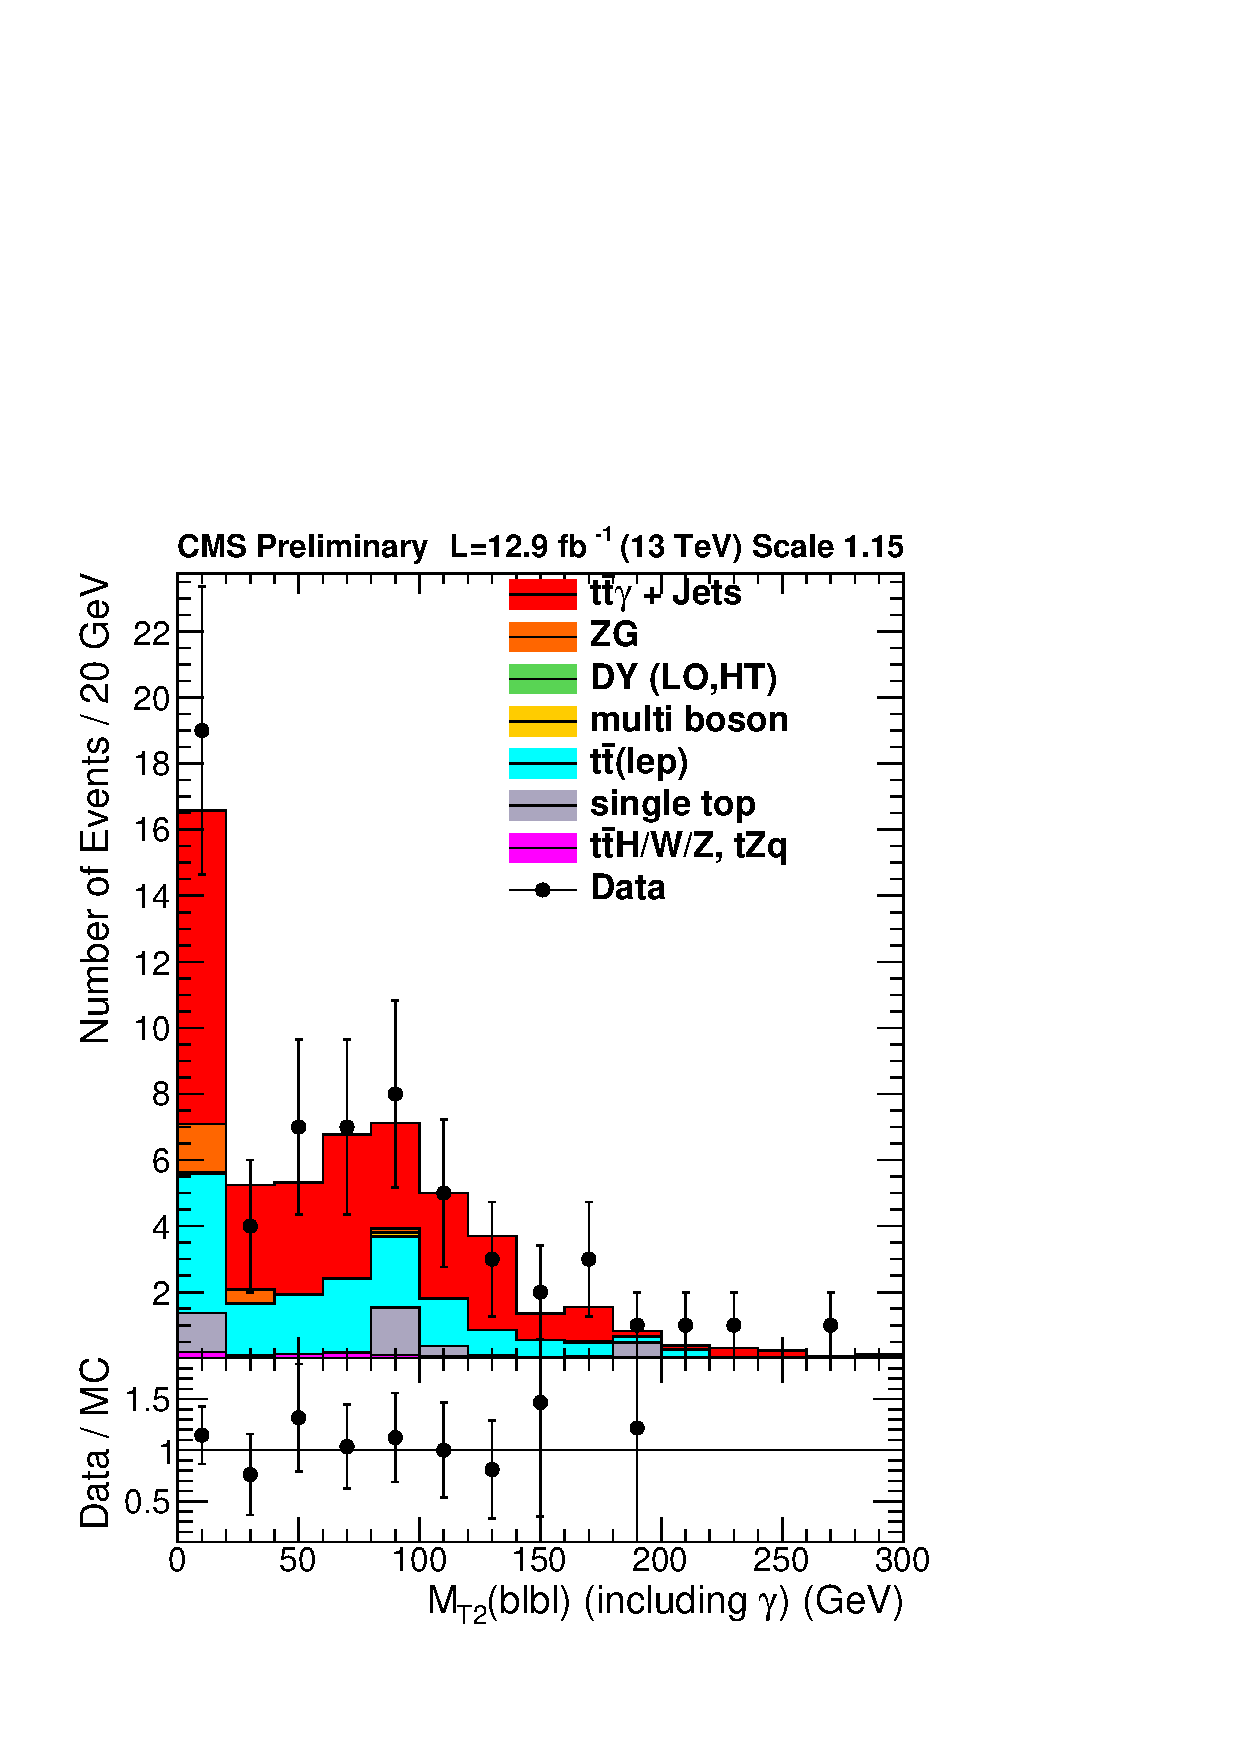
\includegraphics[width=0.45\textwidth]{figures/TTG/all/njet2-photon30-llgNoZ-gJetdR-gLepdR-btagM-mll20-met80-metSig5-dPhiJet0-dPhiJet1/dl_mt2blbl_photonEstimated.pdf}}
      \subfloat[other MC subtracted]{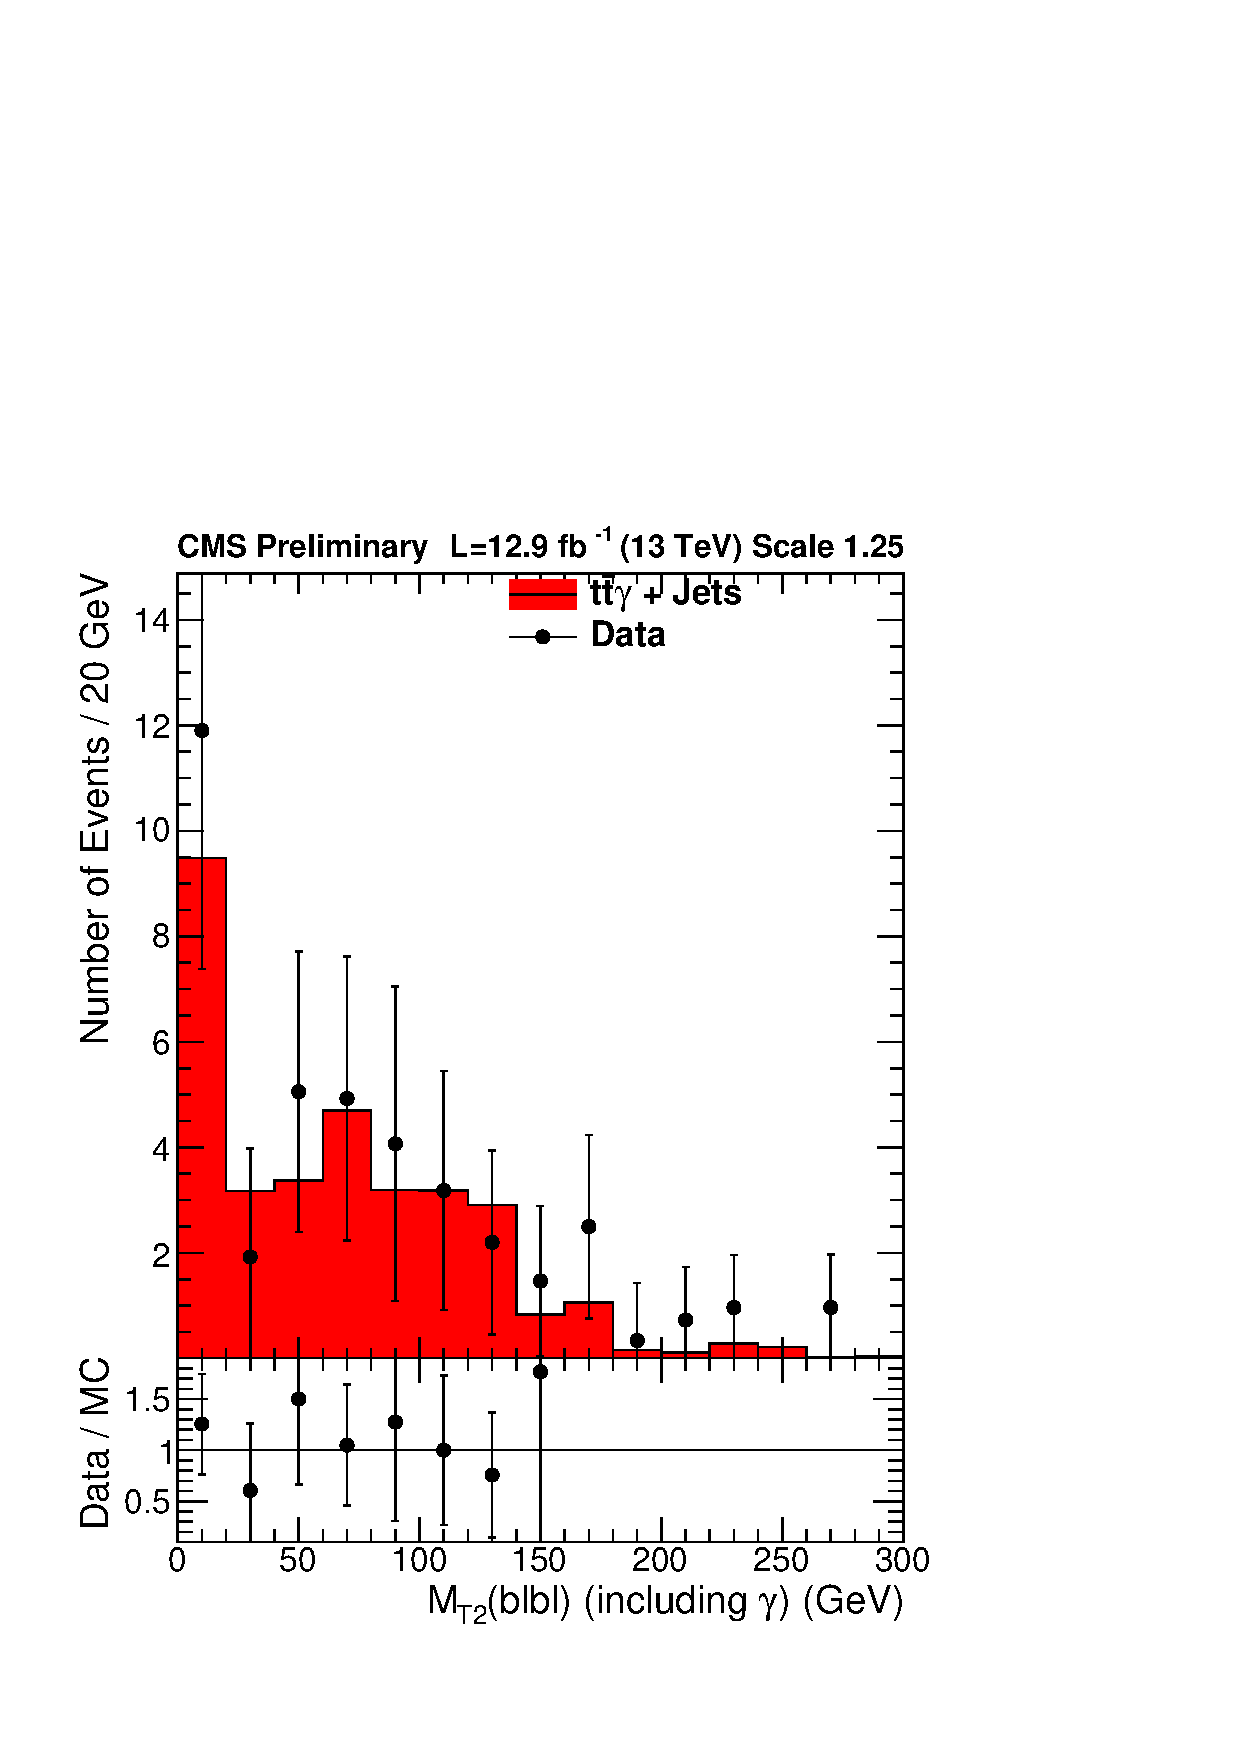
\includegraphics[width=0.45\textwidth]{figures/TTG_subtracted/all/njet2-photon30-llgNoZ-gJetdR-gLepdR-btagM-mll20-met80-metSig5-dPhiJet0-dPhiJet1/dl_mt2blbl_photonEstimated.pdf}}
      \caption{Distribution of \mtlblb using the photon-estimated \metPhoton (after \met cuts)}
      \label{fig:ttg_mt2blbl}
    \end{figure}

    \begin{figure}
      \centering
      \subfloat[other MC included]{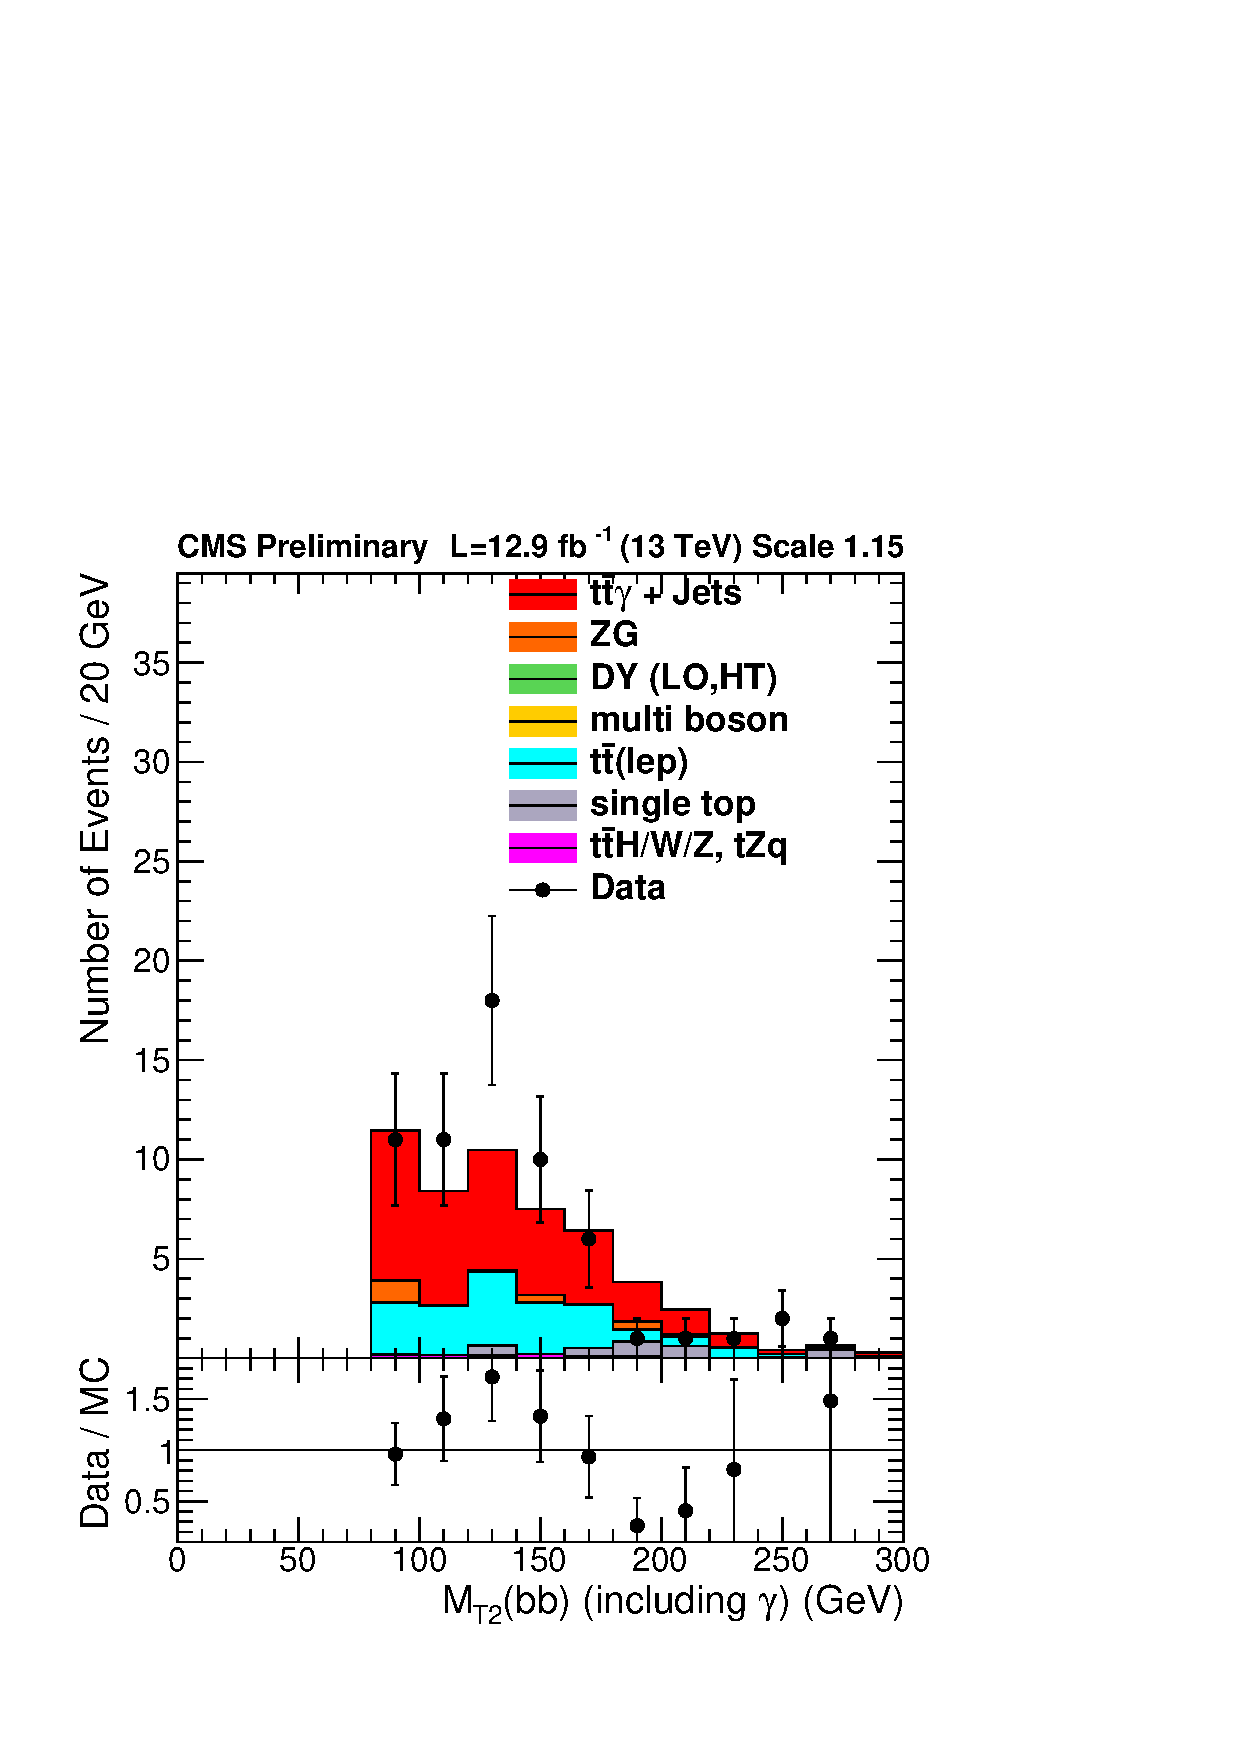
\includegraphics[width=0.45\textwidth]{figures/TTG/all/njet2-photon30-llgNoZ-gJetdR-gLepdR-btagM-mll20-met80-metSig5-dPhiJet0-dPhiJet1/dl_mt2bb_photonEstimated.pdf}}
      \subfloat[other MC subtracted]{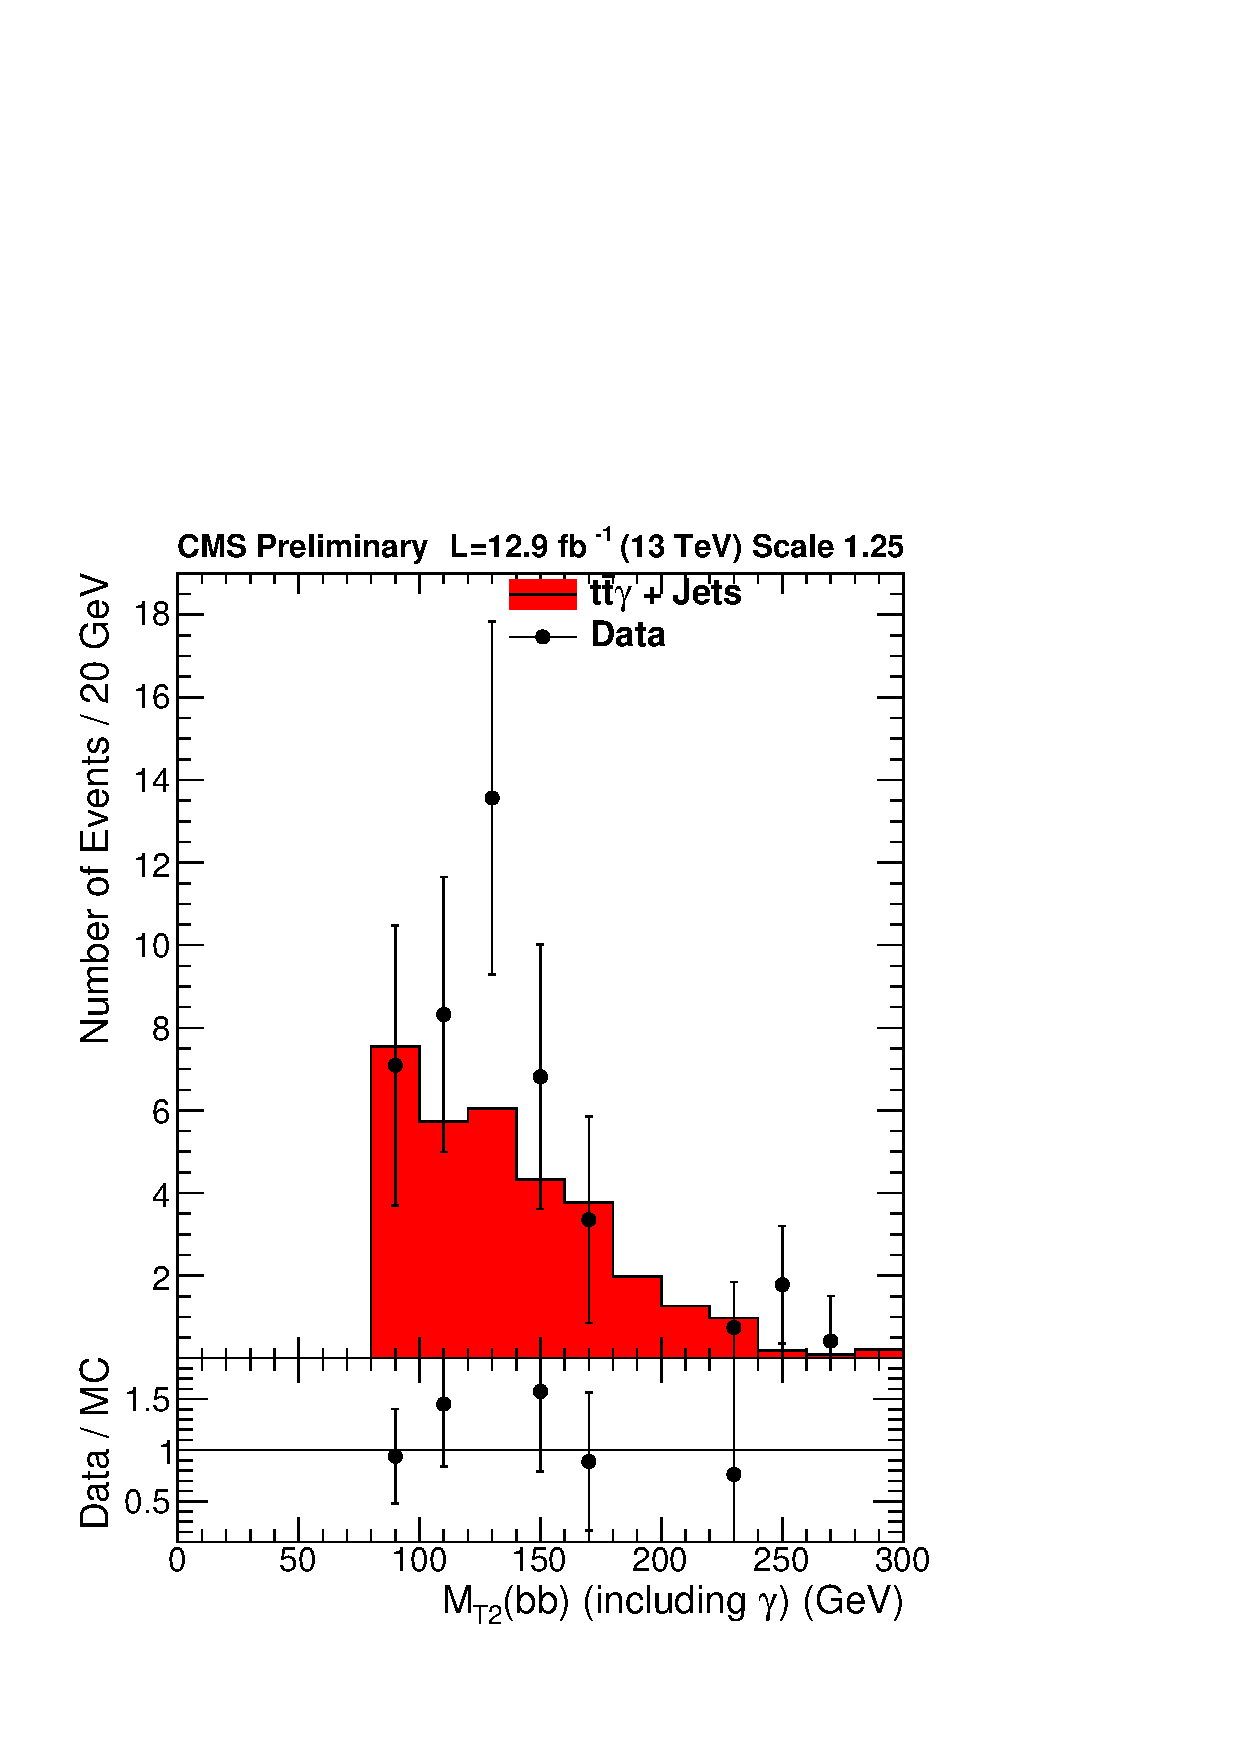
\includegraphics[width=0.45\textwidth]{figures/TTG_subtracted/all/njet2-photon30-llgNoZ-gJetdR-gLepdR-btagM-mll20-met80-metSig5-dPhiJet0-dPhiJet1/dl_mt2bb_photonEstimated.pdf}}
      \caption{Distribution of \mtbb using the photon-estimated \metPhoton (after \met cuts)}
      \label{fig:ttg_mt2bb}
    \end{figure}
